% !TEX program = xelatex
% ============================================================
%  全国大学生数学建模竞赛 (CUMCM) LaTeX 通用论文模板
%  编译方式: XeLaTeX
% ============================================================
\documentclass[12pt,a4paper]{ctexart}

% ======================== 宏包加载 ========================
\usepackage[top=2.5cm, bottom=2.5cm, left=2.8cm, right=2.8cm]{geometry}
\usepackage{amsmath, amssymb, amsthm}
\usepackage{graphicx}
\usepackage{float}
\usepackage{subcaption}
\usepackage{booktabs}
\usepackage{array}
\usepackage{multirow}
\usepackage{longtable}
\usepackage{xcolor}
\usepackage{hyperref}
\hypersetup{
    colorlinks=true,
    linkcolor=blue!70!black,
    citecolor=green!50!black,
    urlcolor=blue!60!black
}
\usepackage{listings}
\lstset{
    basicstyle=\small\ttfamily,
    breaklines=true,
    frame=single,
    numbers=left,
    numberstyle=\tiny\color{gray},
    keywordstyle=\color{blue},
    commentstyle=\color{green!60!black},
    stringstyle=\color{red!70!black},
    tabsize=4
}

\usepackage{setspace}
\onehalfspacing
\usepackage{enumitem}
\setlist{nosep, leftmargin=2em}
\usepackage{titlesec}
\usepackage{caption}
\usepackage{bm}
\usepackage{mathtools}

% ======================== 字体设置 ========================
\setCJKmainfont{SimSun}[BoldFont=SimHei, ItalicFont=KaiTi]
\setCJKsansfont{SimHei}
\setCJKmonofont{FangSong}
\setmainfont{Times New Roman}
% 显式把 ctex 的 \songti/\heiti/\kaishu/\fangsong 族都配上粗体，避免
% 在摘要等使用 \songti 的环境里 \textbf{中文} 无法加粗（显示不出黑体）。
\setCJKfamilyfont{zhsong}{SimSun}[BoldFont=SimHei]
\setCJKfamilyfont{zhhei}{SimHei}[BoldFont=SimHei]
\setCJKfamilyfont{zhkai}{KaiTi}[BoldFont=SimHei]
\setCJKfamilyfont{zhfang}{FangSong}[BoldFont=SimHei]

% ======================== 编号格式 ========================
\renewcommand{\thesection}{\chinese{section}、}
\renewcommand{\thesubsection}{\arabic{section}.\arabic{subsection}}
\renewcommand{\thesubsubsection}{\arabic{section}.\arabic{subsection}.\arabic{subsubsection}}

% ======================== 标题格式 ========================
\titleformat{\section}
  {\centering\heiti\zihao{-3}\bfseries}
  {\thesection}{0em}{}
\titlespacing*{\section}{0pt}{1.5ex plus .5ex minus .2ex}{1.0ex plus .2ex}

\titleformat{\subsection}
  {\heiti\zihao{4}\bfseries}
  {\thesubsection}{1em}{}
\titlespacing*{\subsection}{0pt}{1.2ex plus .4ex minus .2ex}{0.8ex plus .2ex}

\titleformat{\subsubsection}
  {\heiti\zihao{-4}\bfseries}
  {\thesubsubsection}{1em}{}
\titlespacing*{\subsubsection}{0pt}{1.0ex plus .3ex minus .1ex}{0.6ex plus .1ex}

% ======================== 定理环境 ========================
\theoremstyle{definition}
\newtheorem{definition}{定义}[section]
\newtheorem{assumption}{假设}[section]
\theoremstyle{plain}
\newtheorem{theorem}{定理}[section]
\newtheorem{lemma}{引理}[section]
\newtheorem{proposition}{命题}[section]
\newtheorem{corollary}{推论}[section]
\theoremstyle{remark}
\newtheorem{remark}{注}[section]

% ======================== 自定义命令 ========================
\renewenvironment{abstract}
  {\begin{center}\heiti\zihao{-3}摘\quad 要\end{center}\zihao{-4}\songti}
  {\par\vspace{1em}}

\newcommand{\keywords}[1]{%
  \par\noindent\textbf{关键词：}#1}

\newenvironment{symboltable}
  {\begin{center}\zihao{5}\begin{tabular}{>{\centering\arraybackslash}p{3.5cm} p{7.5cm} >{\centering\arraybackslash}p{1.5cm}}
  \toprule
  \textbf{符号} & \textbf{含义} & \textbf{单位} \\
  \midrule}
  {\bottomrule\end{tabular}\end{center}}

\newcommand{\step}[1]{\par\noindent\textbf{Step #1}\quad}

% ============================================================
\begin{document}
\pagestyle{plain}
\setcounter{page}{1}
\pagenumbering{arabic}
\begin{center}
{\zihao{-2}\heiti\bfseries 我国碳排放数据分析与研究}
\end{center}
\vspace{0.5em}
\begin{center}
\zihao{-4}基于部门排放、省级清单与能源结构驱动变量的统计建模
\end{center}

\begin{abstract}
\noindent\hspace*{2em}碳排放数据分析是识别区域减排差异、研判能源转型路径和支撑双碳政策的重要基础。本文针对我国碳排放的空间差异、能源结构驱动、长期情景预测和政策转译四个问题，基于全国日频分部门排放数据、30省排放清单及统计年鉴驱动变量，采用\textbf{全局Moran检验、PCA可视化与Ward聚类、带符号约束的STIRPAT-ridge和多情景预测}等方法，构建空间画像、结构解释、趋势研判和政策闭环的系列模型。对2025年前三季度数据按2019--2024年同期占全年比例的均值年化，获得全国排放连续性锚点$11639.658\ \mathrm{Mt\ CO_2}$。

\textbf{针对问题一，}本文以排放总量、人均排放、排放强度、煤炭排放占比和过程排放占比构建省级指标体系，利用\textbf{全局Moran检验、PCA二维展示与Ward聚类}识别空间关联和类型差异。省级总量的Moran $I=0.2158$、置换$p=0.061$，在5\%水平不显著；人均排放、排放强度和过程排放占比的Moran $I$分别为$0.3145$、$0.4113$和$0.4073$，置换$p$值均不超过$0.002$。以轮廓系数最大为可复验准则选择$k=3$（轮廓系数$0.3393$），将30个省份划分为高规模高压力型、低规模相对低碳型及其结构差异簇。

\textbf{针对问题二，}以2019--2024年全国年度排放为响应变量，以人口、GDP、煤炭占比和清洁能源比重为解释变量，建立\textbf{带符号约束的STIRPAT-ridge模型}，并以留一法选择岭参数、以严格扩展窗口进行回测。最优岭参数为$0.0429449$；在训练折内独立标准化的严格扩展窗口下，结构模型MAE为$184.397\ \mathrm{Mt}$，高于时间趋势ridge基线的$157.860\ \mathrm{Mt}$。因此，本文将其用于方向受控的结构解释与情景比较，而不宣称其优于纯趋势模型；GDP标准化系数为$0.034528$，清洁能源比重系数为$-0.009301$。

\textbf{针对问题三，}在问题二模型基础上设置基准、低碳和强化低碳三条路径，煤炭占比年下降速度分别取$0.6$、$1.0$和$1.4$个百分点。预测期内总量始终满足\textbf{强化低碳$<$低碳$<$基准}；2045年三种情景的排放总量分别为$12890.561$、$13437.482$和$13864.762\ \mathrm{Mt\ CO_2}$。三条路径的最大值均在2045年预测窗口边界，因而只能判断\textbf{预测窗口内未见达峰，峰值可能在2045年以后}。

\textbf{针对问题四，}本文将省域类型、部门排放结构和情景结果转化为\textbf{“类型识别--部门施策--阶段推进--指标监测”}的政策闭环。针对高规模高压力、效率偏弱和煤炭结构压力等不同情形，分别配置重点行业碳预算、设备更新、非化石能源消纳、储能和需求响应等措施，并按2026--2030年、2031--2035年和2036--2045年分阶段实施，以总量、强度、能源结构、部门排放和数据质量指标开展年度复盘。
\end{abstract}

\keywords{碳排放分析；空间集聚；PCA可视化与Ward聚类；STIRPAT-ridge；情景预测；双碳政策}

\section{问题重述与问题分析}

\subsection{问题重述}
题目要求利用全国日频分部门排放数据、30个省份排放清单和统计年鉴变量，完成四项相互衔接的任务：其一，识别省级排放的空间差异并完成分类分级；其二，识别人口、经济规模与能源结构对全国碳排放的统计关联，建立具有预测能力的模型；其三，设置不同低碳转型路径，预测2026--2045年的排放总量、排放强度及达峰特征；其四，将上述结果转化为分区域、分部门、分阶段的建议。本文严格区分省级横截面清单和全国时间序列，避免将不同统计口径直接拼接。

\subsection{数据口径与任务对应}
附件1覆盖2019年1月1日至2025年9月30日，共17255条部门--日期记录，包含全国总量\texttt{Total}和六类部门记录\cite{data1}；附件2提供30个省级清单，省级总量采用\texttt{Scope\_1\_Total}，不含西藏\cite{data2}。人口、GDP、煤炭比重和清洁能源比重取自国家统计局年鉴相应表项\cite{stats}。主要数据及其在各问题中的作用见表\ref{tab:data}。

\begin{table}[H]
\centering
\caption{数据集、统计口径及模型用途}
\label{tab:data}
\zihao{5}
\begin{tabular}{>{\raggedright\arraybackslash}p{2.6cm}>{\raggedright\arraybackslash}p{4.3cm}>{\raggedright\arraybackslash}p{5.4cm}}
\toprule
数据集 & 规模与口径 & 用途\\
\midrule
附件1：全国日频排放数据 & 2019--2025年、2465个日期、7类部门；单位为Mt CO$_2$ & 部门结构核验、年度总量、2025年年化锚点与问题二响应变量\\
附件2：省级排放清单 & 30个省份、\texttt{Scope\_1\_Total}；单位为Mt CO$_2$ & 省级规模、强度、人均排放、空间检验与聚类分类\\
统计年鉴驱动变量 & 2019--2024年人口、GDP、煤炭比重、清洁能源比重 & STIRPAT-ridge建模与三情景外生路径设定\\
项目结果文件 & CSV、JSON、PNG/SVG与复现清单 & 参数核对、图表制备、回测与情景约束验证\\
\bottomrule
\end{tabular}
\end{table}

\subsection{问题分析与总体技术路线}
问题一的核心是横截面差异而非时间预测，因此以省级标准化指标、空间自相关和聚类画像回答“哪些指标具有空间集聚、哪些地区应优先治理”。问题二的年度样本只有6期，若直接使用无约束多元回归，容易出现与能源转型机理相反的系数方向；故以带符号约束的岭回归稳定估计并用训练折内独立标准化的扩展窗口检验外推误差。问题三将经回测的结构模型与外生情景路径连接，以总量和强度双指标进行比较；问题四不再引入未经数据支撑的优化参数，而是把省域类别、部门排放、模型方向和情景差异映射为可监测的治理工具。技术路线可概括为“口径核验--空间画像--结构模型--情景预测--政策闭环”。

\subsection{输出口径与验证安排}
四个问题的输出对象和验证方式不同。问题一输出空间自相关统计量、聚类数选择和省级类别，验证重点是空间权重、置换次数、标准化过程与聚类准则是否透明；问题二输出符号受控的系数、岭参数和外推误差，验证重点是训练--测试顺序不能泄露未来数据；问题三输出情景路径、年度总量、强度和约束检查，验证重点是每个情景都满足人口、GDP和能源占比的边界条件；问题四输出省级工具标识、类别覆盖率、部门优先级和阶段指标，验证重点是政策图表能否由问题一至问题三的真实结果重新计算。

因此，本文不把“模型拟合较好”作为所有问题的统一标准。空间问题关注显著性与分组的可解释性，预测问题关注严格外推误差和情景约束，政策问题关注规则的透明性和指标的可监测性。所有数值均保留在\texttt{results}目录：问题一对应Moran检验、聚类决策与省级分类表；问题二对应系数和回测表；问题三对应63行预测和路径约束表；问题四对应省级映射、类别覆盖率、部门优先级和阶段情景指标。这样的分层安排避免了用单一误差指标去替代政策建议的可追溯性。
\section{模型假设、符号与数据预处理}

\subsection{模型假设}
为使不同来源的数据能够在明确边界内使用，作如下假设：
\begin{enumerate}[label=(\arabic*)]
\item 附件1中的\texttt{Total}等于国内航空、地面交通、工业、电力和居民五部门之和；国际航空作为单列展示项，不重复计入该恒等式。
\item 2025年1--9月的季节性与2019--2024年同期比例的均值具有可比性，因此年化值只作为模型衔接锚点，不视为已发布的完整年度统计。
\item 省界相邻可近似刻画省级空间联系；海南采用与广东、广西的桥接关系，故空间检验仅用于探索性识别，不推断局部因果。
\item 人口、GDP和煤炭相关占比对排放的方向约束为非负，清洁能源比重约束为非正；约束表达的是建模先验，不等同于因果识别。
\item 2026--2045年外生路径只代表本文设定的情景，不等同于任何官方规划；情景预测不确定性通过残差参考带提示，但不解释为严格置信区间。
\end{enumerate}

\subsection{符号说明}
主要符号见表\ref{tab:symbol}。省级强度与全国预测强度使用的GDP单位不同，本文在对应章节中分别标注，避免将$t/(万元\ GDP)$与$\mathrm{Mt}/(万亿元\ GDP)$混用。

\begin{table}[H]
\centering
\caption{主要符号及含义}
\label{tab:symbol}
\zihao{5}
\begin{tabular}{>{\centering\arraybackslash}p{2.7cm}>{\raggedright\arraybackslash}p{7.2cm}>{\centering\arraybackslash}p{2.0cm}}
\toprule
符号 & 含义 & 单位\\
\midrule
$C_t$ & 第$t$年全国二氧化碳排放量 & Mt CO$_2$\\
$E_i$ & 第$i$个省份排放规模 & Mt CO$_2$\\
$PC_i$ & 第$i$个省份人均排放 & t/person\\
$EI_i$ & 第$i$个省份单位GDP排放强度 & t/(万元 GDP)\\
$S_t^{coal}$、$S_t^{clean}$ & 全国煤炭比重、清洁能源比重 & $[0,1]$\\
$P_t$、$G_t$ & 全国人口、GDP & 万人、万亿元\\
$w_{ij}$ & 省份$i$与$j$之间的空间权重 & 无量纲\\
$\lambda$ & 岭回归正则化参数 & 无量纲\\
$I_t^{GDP}$ & 全国排放强度$C_t/G_t$ & Mt/(万亿元 GDP)\\
\bottomrule
\end{tabular}
\end{table}

\subsection{口径核验与年化处理}
对附件1逐日核验\texttt{Total}与五个国内部门之和，最大绝对误差为$2.0\times10^{-6}$ Mt，属于浮点计算精度范围。2025年仅含前三季度，令$f_y$为历史年份1--9月排放占全年比例，则年化锚点定义为
\begin{equation}
f_y=\frac{C_{y,1\text{--}9}}{C_{y,1\text{--}12}},\qquad
\widehat C_{2025}=\frac{C_{2025,1\text{--}9}}{\frac{1}{6}\sum_{y=2019}^{2024}f_y}=11639.658\ \mathrm{Mt\ CO_2}.
\label{eq:annualize}
\end{equation}
历史同期比例均值为$0.740197$、标准差为$0.011311$，表明年化过程中采用的季节比例在样本内波动较小。该值用于问题二和问题三的连续性连接，不能替代官方年度总量。

\subsection{数据预处理与质量控制}
全国日频数据先按日期和部门汇总为年度序列，再保留2019--2024年的已完整年度用于估计；2025年只作为式\eqref{eq:annualize}得到的锚点进入情景衔接。该处理避免把未完整年度与完整年度共同用于回归而引入系统性偏差。省级清单按工作表读取后，统一省名并与GDP、人口字典进行一一匹配；对省名、样本数量、GDP、人口及\texttt{Scope\_1\_Total}均进行完整性断言。因省级清单不含西藏，后续的$n=30$只对应这30个可核验省级单元。

针对尺度差异，排放规模直接保留Mt单位用于排名和重点治理判定，人均排放和强度分别按式\eqref{eq:q1-indicator}计算；进入PCA和聚类之前，对五项特征先进行$\log(1+x)$变换，再进行标准化。对数变换降低了少数高规模省份对欧氏距离的支配作用，标准化则使总量、比例和强度在Ward距离中具有相同的初始权重。需要强调的是，经济联系指数是强度、煤炭占比和过程排放占比标准化值的均值，只在问题四的市场机制触发规则中使用，不被解释为真实的跨省贸易流或能源流。

为方便复查，输入哈希、随机种子20260822、置换次数999、年化方法和复现命令均写入\texttt{results/复现清单.json}。全量运行前后，附件1总量恒等式的最大绝对误差均为$2.0\times10^{-6}$ Mt；该误差远小于年度排放量数量级，故保留为浮点计算误差记录而不进行人为修正。
\section{问题一：省级空间差异识别与分类分级}

\subsection{指标构建与空间权重}
对附件2的30个省份分别计算排放规模、人均排放、排放强度、煤炭排放占比和过程排放占比。人口单位为万人、GDP单位为亿元，故人均排放和排放强度写为
\begin{equation}
PC_i=\frac{100E_i}{Pop_i},\qquad EI_i=\frac{100E_i}{GDP_i}.
\label{eq:q1-indicator}
\end{equation}
空间权重采用省界相邻的0--1矩阵；为避免孤立单元，海南与广东、广西建立桥接。该设定可复现但并不代表真实能源流网络，因此后文只报告全局空间关联证据。

\subsection{全局Moran检验}
对每项指标计算全局Moran's $I$\cite{moran}：
\begin{equation}
I=\frac{n}{S_0}\frac{\sum_i\sum_jw_{ij}(x_i-\bar x)(x_j-\bar x)}{\sum_i(x_i-\bar x)^2},\qquad S_0=\sum_i\sum_jw_{ij},
\label{eq:moran}
\end{equation}
并以999次固定种子置换计算双侧经验$p$值。原始排放规模排序如图\ref{fig:q1-raw}所示，规模、人均和强度之间的关系见图\ref{fig:q1-process}；检验结果列于表\ref{tab:moran}。

\begin{figure}[H]
\centering
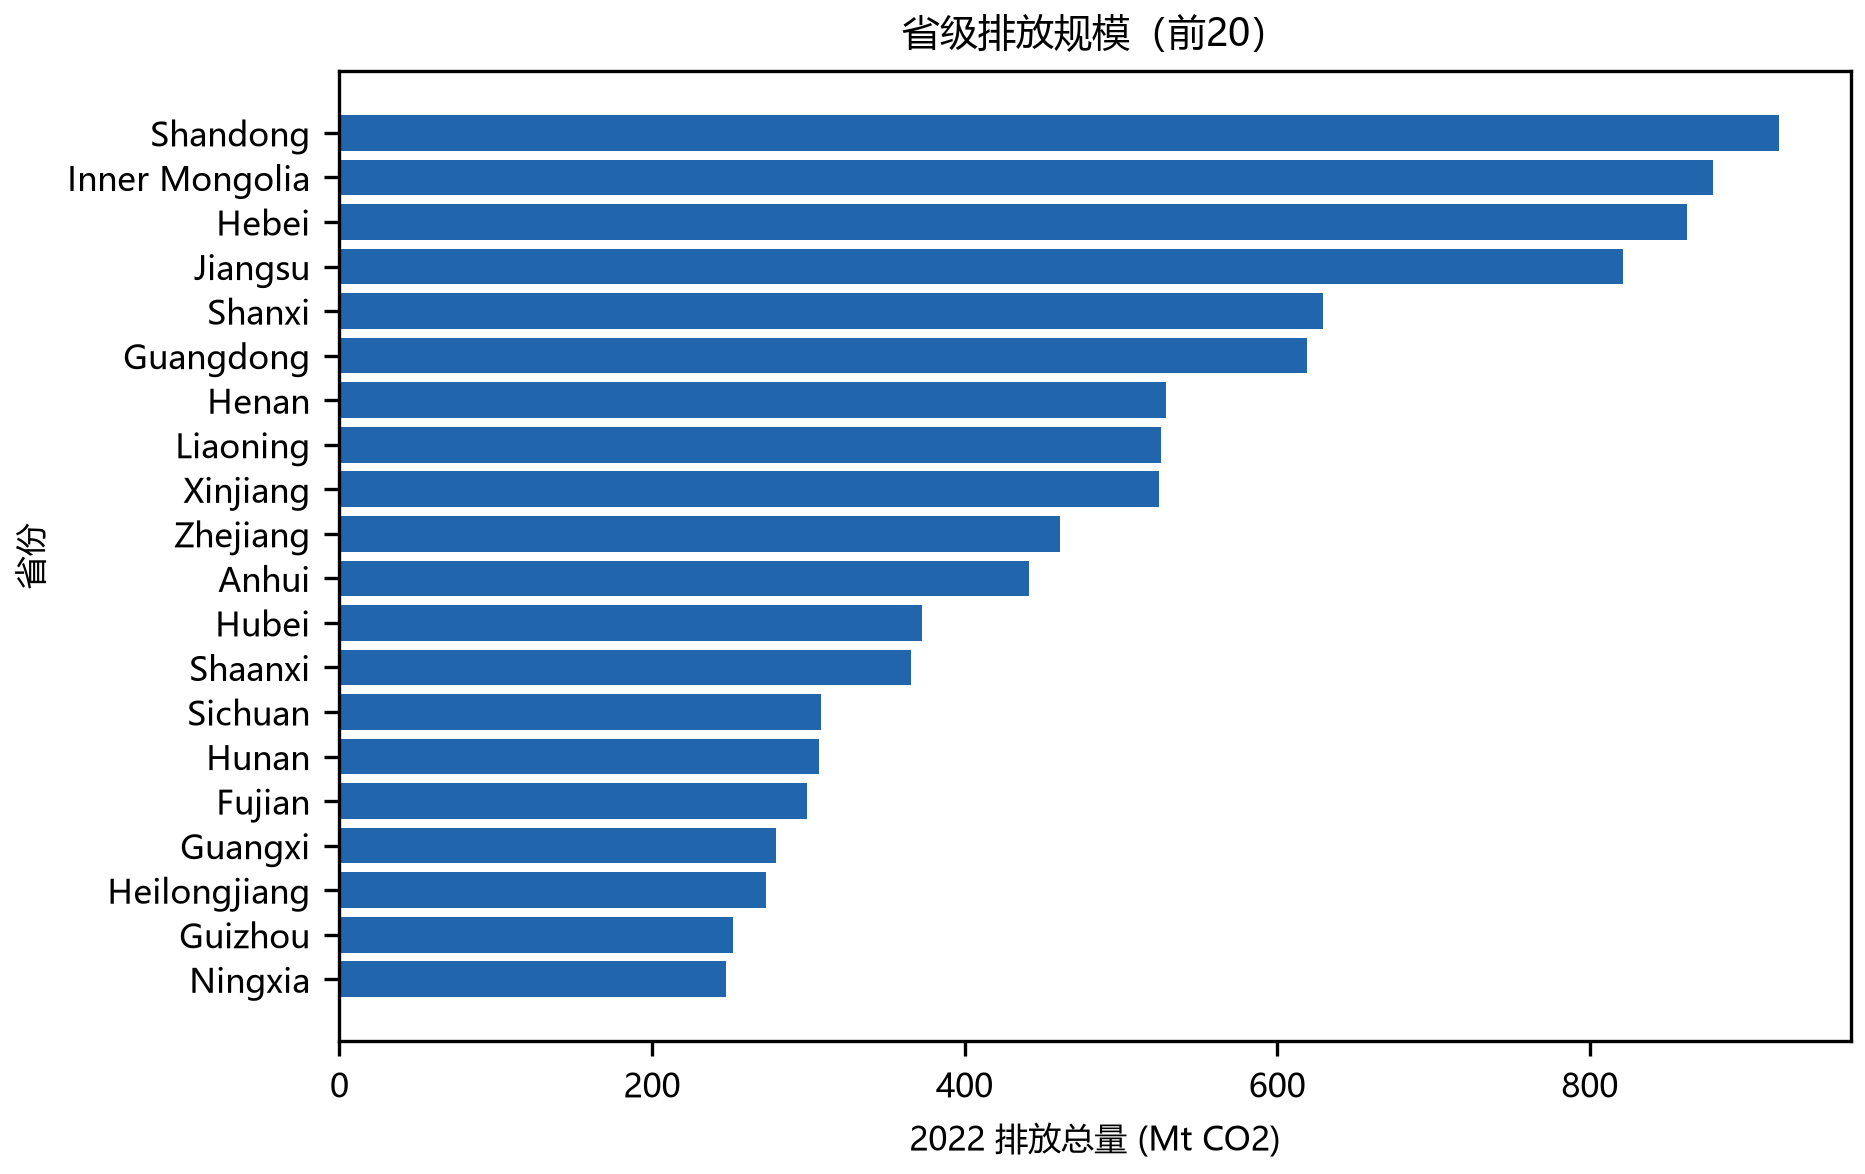
\includegraphics[width=0.86\textwidth]{figures/raw_q1_province_scale.png}
\caption{2022年省级排放规模前20省份}
\label{fig:q1-raw}
\end{figure}

\begin{figure}[H]
\centering
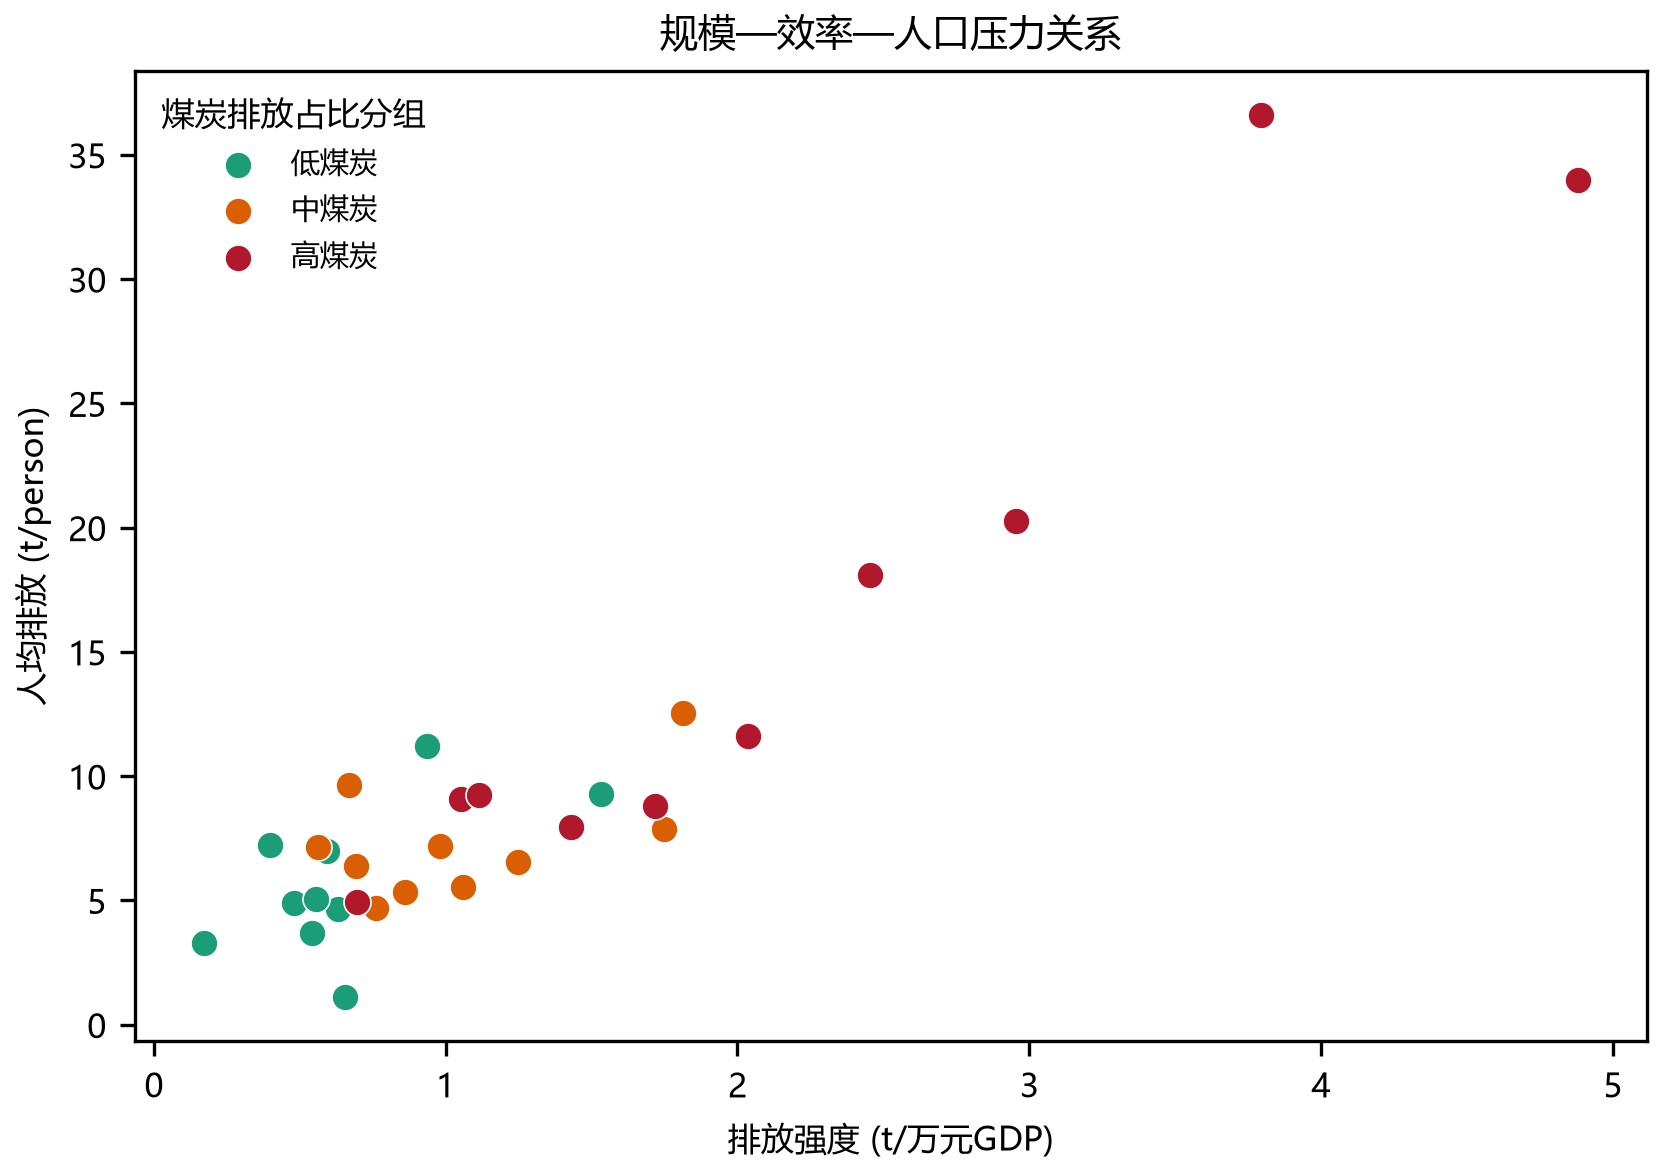
\includegraphics[width=0.80\textwidth]{figures/process_q1_indicator_space.png}
\caption{省级排放规模、效率、人口压力与能源结构关系}
\label{fig:q1-process}
\end{figure}

\begin{table}[H]
\centering
\caption{省级指标的全局Moran检验结果}
\label{tab:moran}
\zihao{5}
\begin{tabular}{lrrl}
\toprule
指标 & Moran $I$ & 置换$p$值 & 5\%水平判断\\
\midrule
排放总量 & 0.2158 & 0.061 & 不显著\\
人均排放 & 0.3145 & 0.002 & 显著\\
排放强度 & 0.4113 & 0.001 & 显著\\
煤炭排放占比 & 0.1735 & 0.100 & 不显著\\
过程排放占比 & 0.4073 & 0.001 & 显著\\
\bottomrule
\end{tabular}
\end{table}

表\ref{tab:moran}显示，省级总量在5\%水平未呈现显著空间集聚，而排放强度、过程排放占比和人均排放存在显著集聚。这意味着区域治理不能只按总量排序：效率、人口压力和工业过程属性更能揭示相邻地区的共同问题。补充的Kruskal--Wallis检验中，煤炭排放占比的$p=0.0522$接近但未达到5\%阈值，其余指标组间差异也未达到显著水平，因而分类结果用于画像与政策分层，不作为严格的统计分割结论。

\subsection{空间检验与优先级识别步骤}
空间检验按以下顺序实施。第一步，依据省界相邻关系建立对称的0--1权重矩阵$W$，并对海南采用桥接关系，保证每一个省份都有可比较的相邻单元。第二步，对总量、人均、强度、煤炭占比和过程排放占比分别按式\eqref{eq:moran}计算观测Moran $I$。第三步，固定随机种子后对每个指标置换999次，形成零假设下的统计量分布；经验$p$值按“置换统计量绝对值不小于观测绝对值”的频率计算。该过程比直接套用正态近似更适合30个省份的小样本情形。

Moran检验回答的是“相邻地区是否具有相似的指标取值”，并不回答“某省份排放是否高”。因此，重点治理对象另按规模和强度的80\%分位数判定：
\begin{equation}
P_i=\mathbb{I}\left\{E_i\geq Q_{0.8}(E)\ \text{或}\ EI_i\geq Q_{0.8}(EI)\right\}.
\label{eq:priority}
\end{equation}
其中$P_i=1$表示重点治理。该规则得到9个重点治理省份，且与聚类标签同时保留在\texttt{问题1\_省级指标与分类.csv}中。由此，空间统计、类别画像和重点判定并非相互替代：前者提供集聚证据，中者提供多指标分组，后者提供可执行的优先级清单。

Kruskal--Wallis检验作为辅助诊断，用总量四分位组比较人均、强度、煤炭占比和过程占比的总体差异。其结果没有被用于制造显著性结论，而是用于提醒读者：煤炭占比的$p=0.0522$接近5\%阈值，但仍不应表述为显著；其他指标的组间$p$值更高。这个限制解释了为什么本文将问题一结果定位为探索性的空间画像和政策分层，而不是确定性的区域因果分类。
\subsection{PCA二维展示、Ward聚类与重点治理识别}
为消除量纲差异，先对五项指标进行标准化；主成分分析仅用于二维可视化，Ward层次聚类则直接在完整的五维标准化特征空间中实施\cite{ward}。前两个主成分解释率分别为53.57\%和26.18\%，二维展示覆盖79.75\%方差。候选聚类数的轮廓系数见表\ref{tab:silhouette}。本文采用唯一的、可审计的选择规则：在$k=2,\ldots,6$中取轮廓系数最大者，若并列则取较小的$k$。因此选择$k=3$，对应轮廓系数0.3393；不再把四级分类作为未经量化的附加理由。

\begin{table}[H]
\centering
\caption{候选聚类数的轮廓系数与选择结果}
\label{tab:silhouette}
\zihao{5}
\begin{tabular}{cccccc}
\toprule
$k$ & 2 & 3 & 4 & 5 & 6\\
\midrule
轮廓系数 & 0.3129 & 0.3393 & 0.2572 & 0.2648 & 0.2639\\
是否选取 & 否 & 是 & 否 & 否 & 否\\
\bottomrule
\end{tabular}
\end{table}

三类省份的数量与代表性省份见表\ref{tab:cluster}，标准化画像见图\ref{fig:q1-result}。高规模高压力型有8个省份，低规模相对低碳型有21个省份，另有1个结构差异簇。总量或强度进入样本前20\%的9个省份被标记为重点治理对象；该标记与聚类类别共同进入问题四的政策映射。

\begin{table}[H]
\centering
\caption{省级分类结果及其可追溯政策含义}
\label{tab:cluster}
\zihao{5}
\begin{tabular}{>{\raggedright\arraybackslash}p{3.4cm}c>{\raggedright\arraybackslash}p{4.6cm}>{\raggedright\arraybackslash}p{3.0cm}}
\toprule
类别 & 数量 & 代表性省份 & 主要治理含义\\
\midrule
高规模高压力型 & 8 & 内蒙古、宁夏、山东、山西、新疆、江苏等 & 优先纳入总量控制、能效改造和煤炭替代规则\\
低规模相对低碳型 & 21 & 上海、云南、吉林、四川、天津、安徽等 & 按省级指标触发能效、市场或需求侧工具，避免一刀切\\
低规模相对低碳型（结构差异簇） & 1 & 北京 & 保留独立画像，结合服务业和终端需求特征单独复核\\
\bottomrule
\end{tabular}
\end{table}

\begin{figure}[H]
\centering
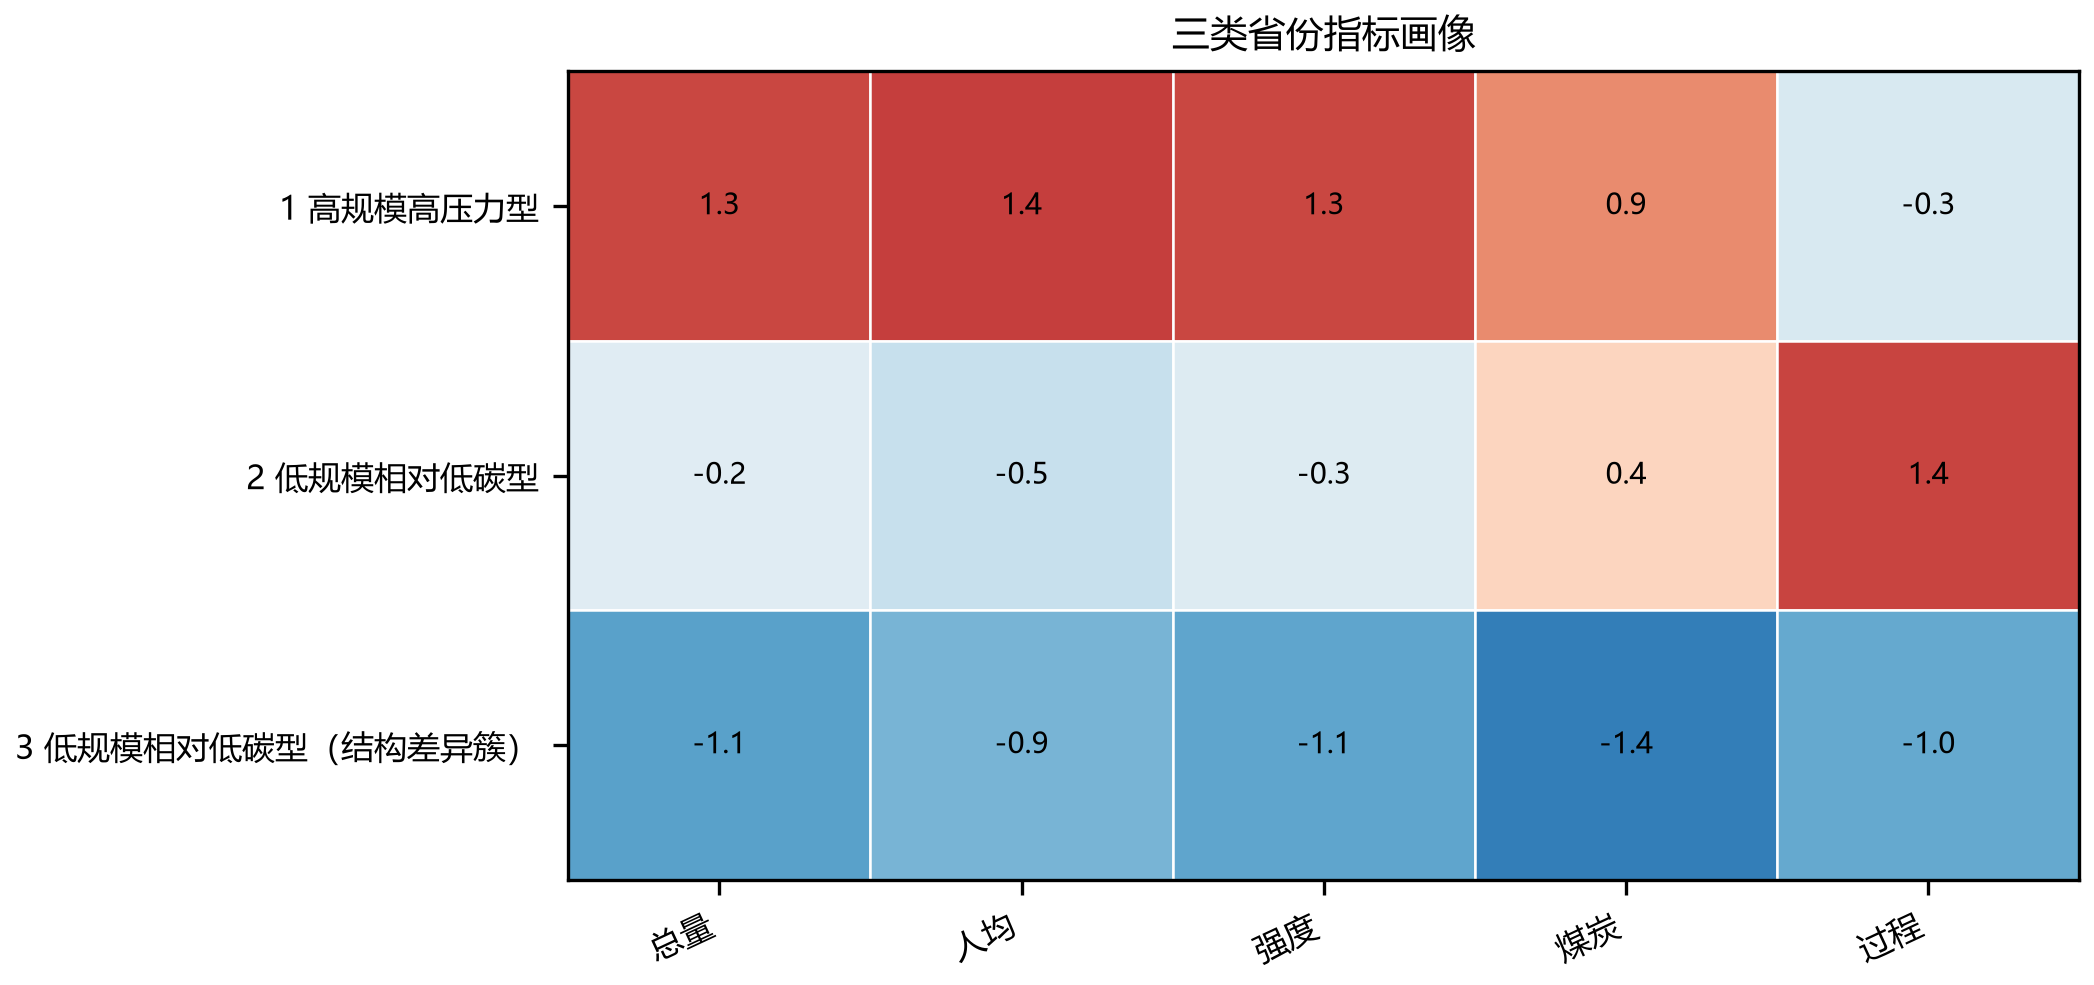
\includegraphics[width=0.90\textwidth]{figures/result_q1_cluster_profile.png}
\caption{三类省份的标准化指标画像}
\label{fig:q1-result}
\end{figure}
\subsection{问题一结果的解释边界}\paragraph{空间结构的读图与决策含义。}
PCA的作用是把五项相关指标压缩为少数综合方向，便于观察省份在“规模--压力”和“结构--效率”上的相对位置。第一主成分解释率为53.57\%，可理解为规模、人均压力与能源结构共同变化的主方向；第二主成分解释率为26.18\%，更多反映排放强度和过程排放占比的差异。这里的“理解”是对载荷方向的统计概括，并不等同于给主成分赋予经济学因果含义。图\ref{fig:q1-process}因而用于展示指标之间的相对关系，不能据此推断某项指标的边际减排效果。

在空间权重方面，本文采用行政区相邻关系，优点是数据获取和复现成本低，且每个省份的邻接关系容易审查；缺点是无法表达跨省电力输送、产业链转移和交通联系。海南的桥接处理仅为避免孤立单元，并不意味着海南与广东或广西之间存在等强度的能源交换。若后续获得经济联系矩阵，可将$w_{ij}$替换为经贸流、能源流或距离衰减权重，并重新报告$I$及其置换分布。也就是说，本文的显著集聚结论应理解为“在相邻权重定义下的空间相关”，而不是对所有网络关系的普遍断言。

重点治理规则还具有一个实际优点：式\eqref{eq:priority}同时保留总量和强度两个入口。当省份总量较大但强度不高时，规则仍可识别其总量控制责任；当省份总量不大但单位产出排放较高时，规则可触发能效改造。该双入口机制避免了仅按总量排序造成的遗漏，也避免把所有低总量地区都归为同一种政策对象。问题四中的政策工具覆盖率正是依据这一省级标记和五类结构条件逐行生成，而不是由聚类标签直接替代。
图\ref{fig:q1-result}展示的是各类指标的标准化平均水平，不是省份间真实排放差额的比例图。高规模高压力型中总量、强度或煤炭结构指标相对更高，因而优先触发总量控制和煤炭替代；低规模相对低碳型的内部仍存在能效、市场机制和需求侧规则的不同触发组合，不能把类别名称理解为“无需治理”。北京形成单独的结构差异簇，提示小规模、低煤炭或服务业主导地区的政策问题可能与资源型地区不同。

聚类数选择同样有边界。轮廓系数只衡量标准化特征空间中的组内紧密与组间分离，不直接评价政策成本、可接受性或减排效果。本文选择$k=3$是因为该准则在候选范围内达到最高值，而不是因为三类恰好对应某种官方行政分级。若未来获得跨省能源流、产业链联系或多年省级清单，可将这些信息用于构造多层权重或面板聚类，并以时间稳定性检验代替单年横截面画像。
\subsection{分类结果的稳健性解释}
聚类结果应从“相对画像”而不是“绝对优劣”理解。首先，输入特征包括排放规模、人均排放、强度、煤炭占比和过程排放占比，它们覆盖了规模、效率、能源与工业过程四个维度，但没有覆盖收入分配、产业链外溢、跨省电力调入调出、气候条件等可能影响排放的变量。其次，Ward方法以欧氏距离合并类别，适合发现总体形状相近的省份，却不会自动识别政策边界。因而，类别名称只是对样本均值的概括，不能替代逐省核查。

其次，轮廓系数选择规则解决的是“在既定特征和算法下选取多少类”的可复验问题，不等于对所有聚类方法的全局最优性声明。若改用不同距离、加入新变量或改用多年面板数据，最佳$k$可能变化。本文将候选范围、轮廓系数、选中标记和规则一并输出，目的在于使审阅者能够复算并在必要时替换选择准则，而不是把一次聚类固化为永久的区域标签。

最后，重点治理标记和类别相互补充。某省可能位于低规模相对低碳型，但因强度进入前20\%而被标记为重点治理；也可能属于高规模高压力型，却在某些工具规则上不满足需求侧条件。政策制定时应先用类别理解共性，再用省级原始指标和式\eqref{eq:priority}确认具体问题，不能只根据类别名称分配资源。
\section{问题二：能源结构驱动模型与预测验证}

\subsection{年度部门结构与建模变量}
问题二使用2019--2024年的全国年度总量作为响应变量，2025年化值仅用于后续连续性校准。图\ref{fig:q2-raw}展示了各部门年度排放变化，说明全国总量具有趋势性且部门结构并非静态。考虑样本容量很小和驱动变量间的共线性，普通最小二乘估计容易不稳定；因此选用带方向约束的岭回归，保留能源结构变量的解释接口。

\begin{figure}[H]
\centering
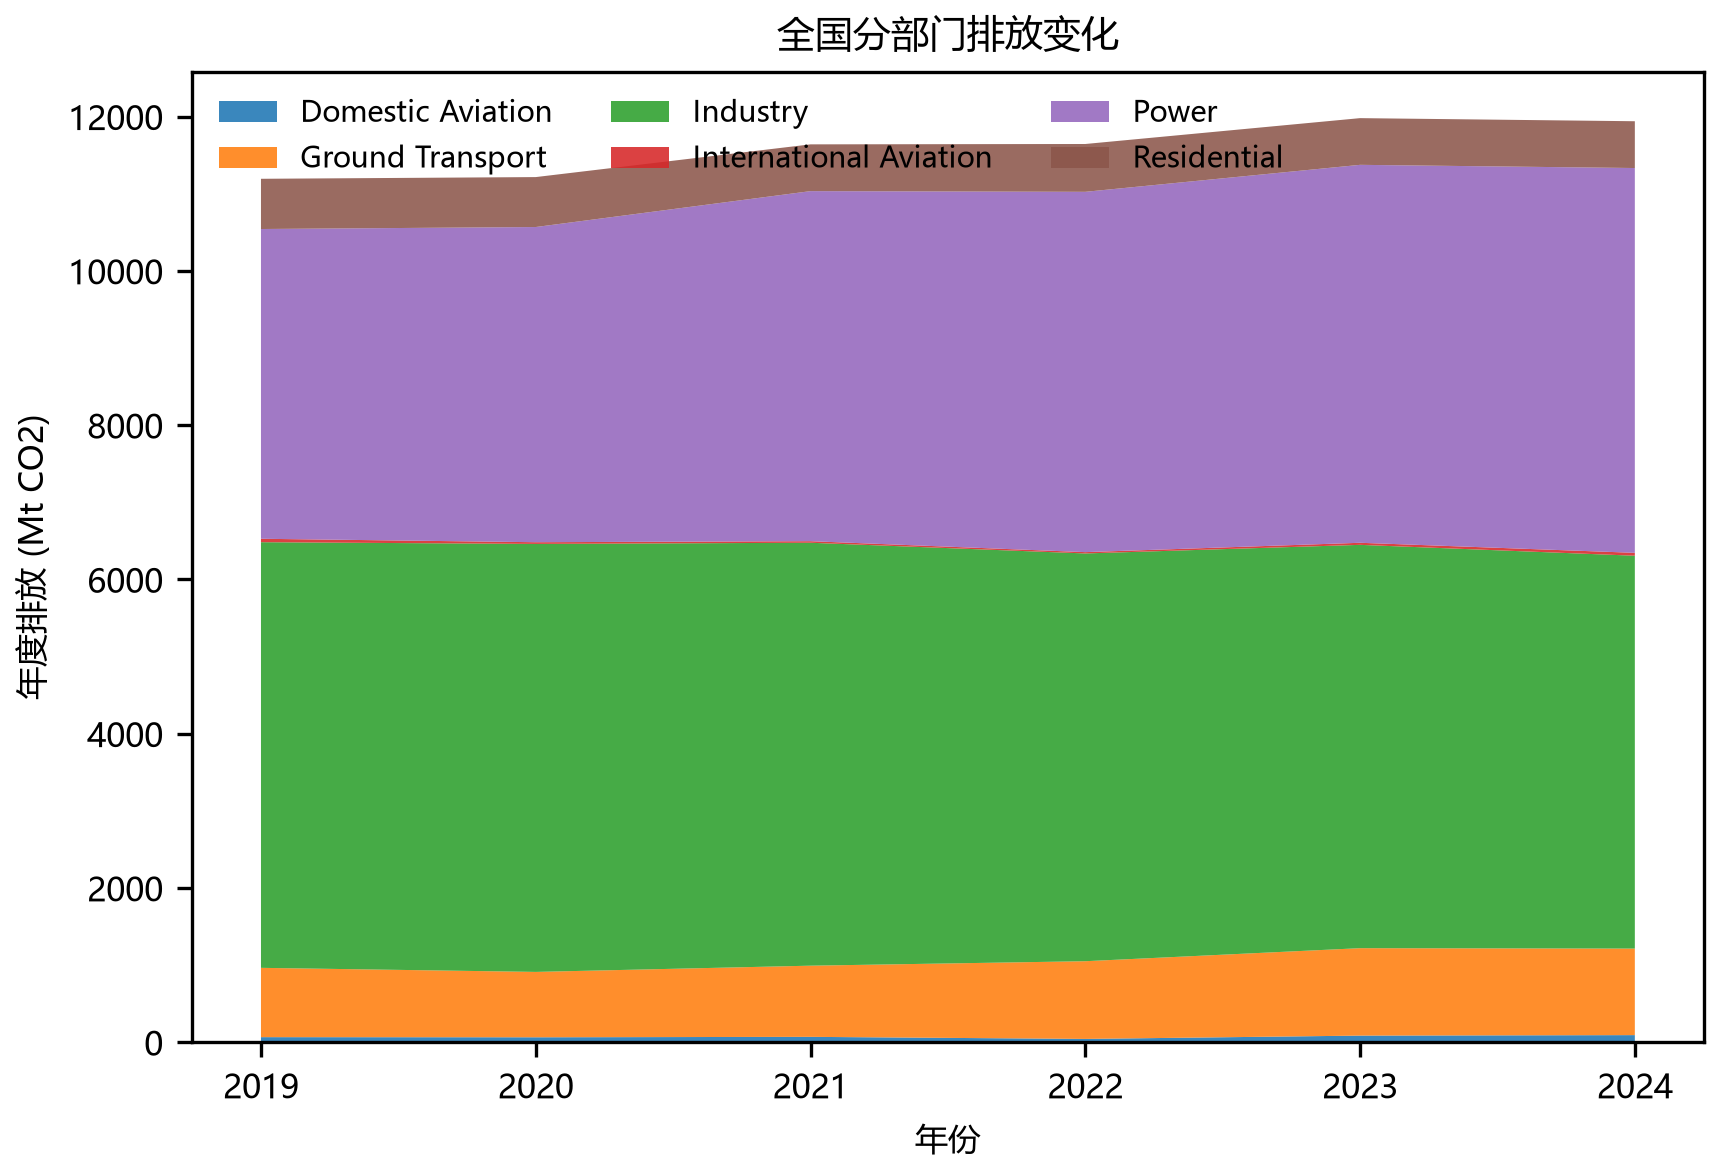
\includegraphics[width=0.86\textwidth]{figures/raw_q2_annual_sectors.png}
\caption{2019--2025年全国分部门排放变化}
\label{fig:q2-raw}
\end{figure}

\subsection{带符号约束的STIRPAT-ridge模型}
STIRPAT将IPAT关系写为可估计的对数回归形式\cite{stirpat}：
\begin{equation}
\ln C_t=\beta_0+\beta_1\ln P_t+\beta_2\ln G_t+\beta_3\ln S_t^{coal}+\beta_4\ln S_t^{clean}+\varepsilon_t.
\label{eq:stirpat}
\end{equation}
在标准化特征上加入$L_2$正则，并施加方向约束：
\begin{equation}
\min_{\bm\beta}\ \|\bm y-\bm X\bm\beta\|_2^2+\lambda\|\bm\beta_{1:4}\|_2^2,\quad
\beta_1,\beta_2,\beta_3\geq0,\quad\beta_4\leq0.
\label{eq:ridge}
\end{equation}
岭回归的正则思想见文献\cite{ridge}。参数$\lambda$采用留一法选择，约束优化由L-BFGS-B实施。该模型并不把短样本系数解释为因果效应，而是提供方向受控的预测结构。

\subsection{参数选择与扩展窗口验证步骤}
模型估计分为参数选择、最终拟合和时间顺序验证三步。第一步，在$10^{-4}$至$10^{4}$的80个对数间隔候选$\lambda$中执行留一年度预测；对每一候选值，轮流删除一个年份；每一折的标准化器仅由剩余年份拟合，再以该变换估计式\eqref{eq:ridge}并预测留出年份，最后计算六次预测的MAE。最小MAE对应$\lambda=0.0429449$。这一过程只用于选择正则化强度，不把留一误差当作最终外推评价。

第二步，使用全部2019--2024年样本和选定$\lambda$重新拟合，得到表\ref{tab:coef}的标准化系数。为避免对系数作过强解释，本文只比较其方向和绝对值相对权重：GDP为正、清洁能源比重为负符合设定的符号先验；人口和煤炭占比落在约束边界，说明在给定6年样本及其他变量后，模型没有为它们分配额外的正向边际系数。该结果不意味着人口或煤炭在现实中没有作用，而是说明短时间序列难以稳定分离共变因素。

第三步，采用严格扩展窗口回测。用2019--2021年预测2022年，再用2019--2022年预测2023年，最后用2019--2023年预测2024年；每一步不仅不允许使用待预测年份的响应变量，也不允许待预测年份参与标准化均值和方差的计算。时间趋势ridge基线使用同一训练窗口、同一正则参数，但只以年份为输入，因此比较回答的是“能源结构模型相对纯趋势模型是否减少外推误差”。表\ref{tab:backtest}给出的184.397 Mt与157.860 Mt正是在这三个外推点上计算；前者较大，说明在本样本下结构模型尚未显示出优于时间趋势基线的外推精度，不能把拟合MAE48.034 Mt误用为前瞻误差。

此外，回测残差的标准差为71.395 Mt。问题三绘制的经验残差范围随预测步长按$\sqrt{h}$放大，用于显示远期预测的不确定性随时间增加；该范围没有模拟参数分布或情景概率，因而在论文中只称为参考带而不称置信区间。
\subsection{系数解释、回测与模型适用边界}
模型系数及相对重要性见表\ref{tab:coef}，图\ref{fig:q2-process}用于呈现系数方向。GDP和清洁能源比重分别保留正、负方向；人口和煤炭占比落在约束边界，因此不能据此声称这两个变量“没有影响”。在该样本中，绝对标准化系数的相对权重定义为
\begin{equation}
\pi_j=100\frac{|\widetilde\beta_j|}{\sum_{k=1}^{4}|\widetilde\beta_k|},
\label{eq:importance}
\end{equation}
其中$\widetilde\beta_j$为标准化特征下的系数。

\begin{table}[H]
\centering
\caption{问题二驱动因素的标准化系数}
\label{tab:coef}
\zihao{5}
\begin{tabular}{lrr}
\toprule
因素 & 标准化系数 & 相对重要性/(\%)\\
\midrule
人口 & 0.000000 & 0.00\\
GDP & 0.034528 & 78.78\\
煤炭占比 & 0.000000 & 0.00\\
清洁能源比重 & -0.009301 & 21.22\\
\bottomrule
\end{tabular}
\end{table}

\begin{figure}[H]
\centering
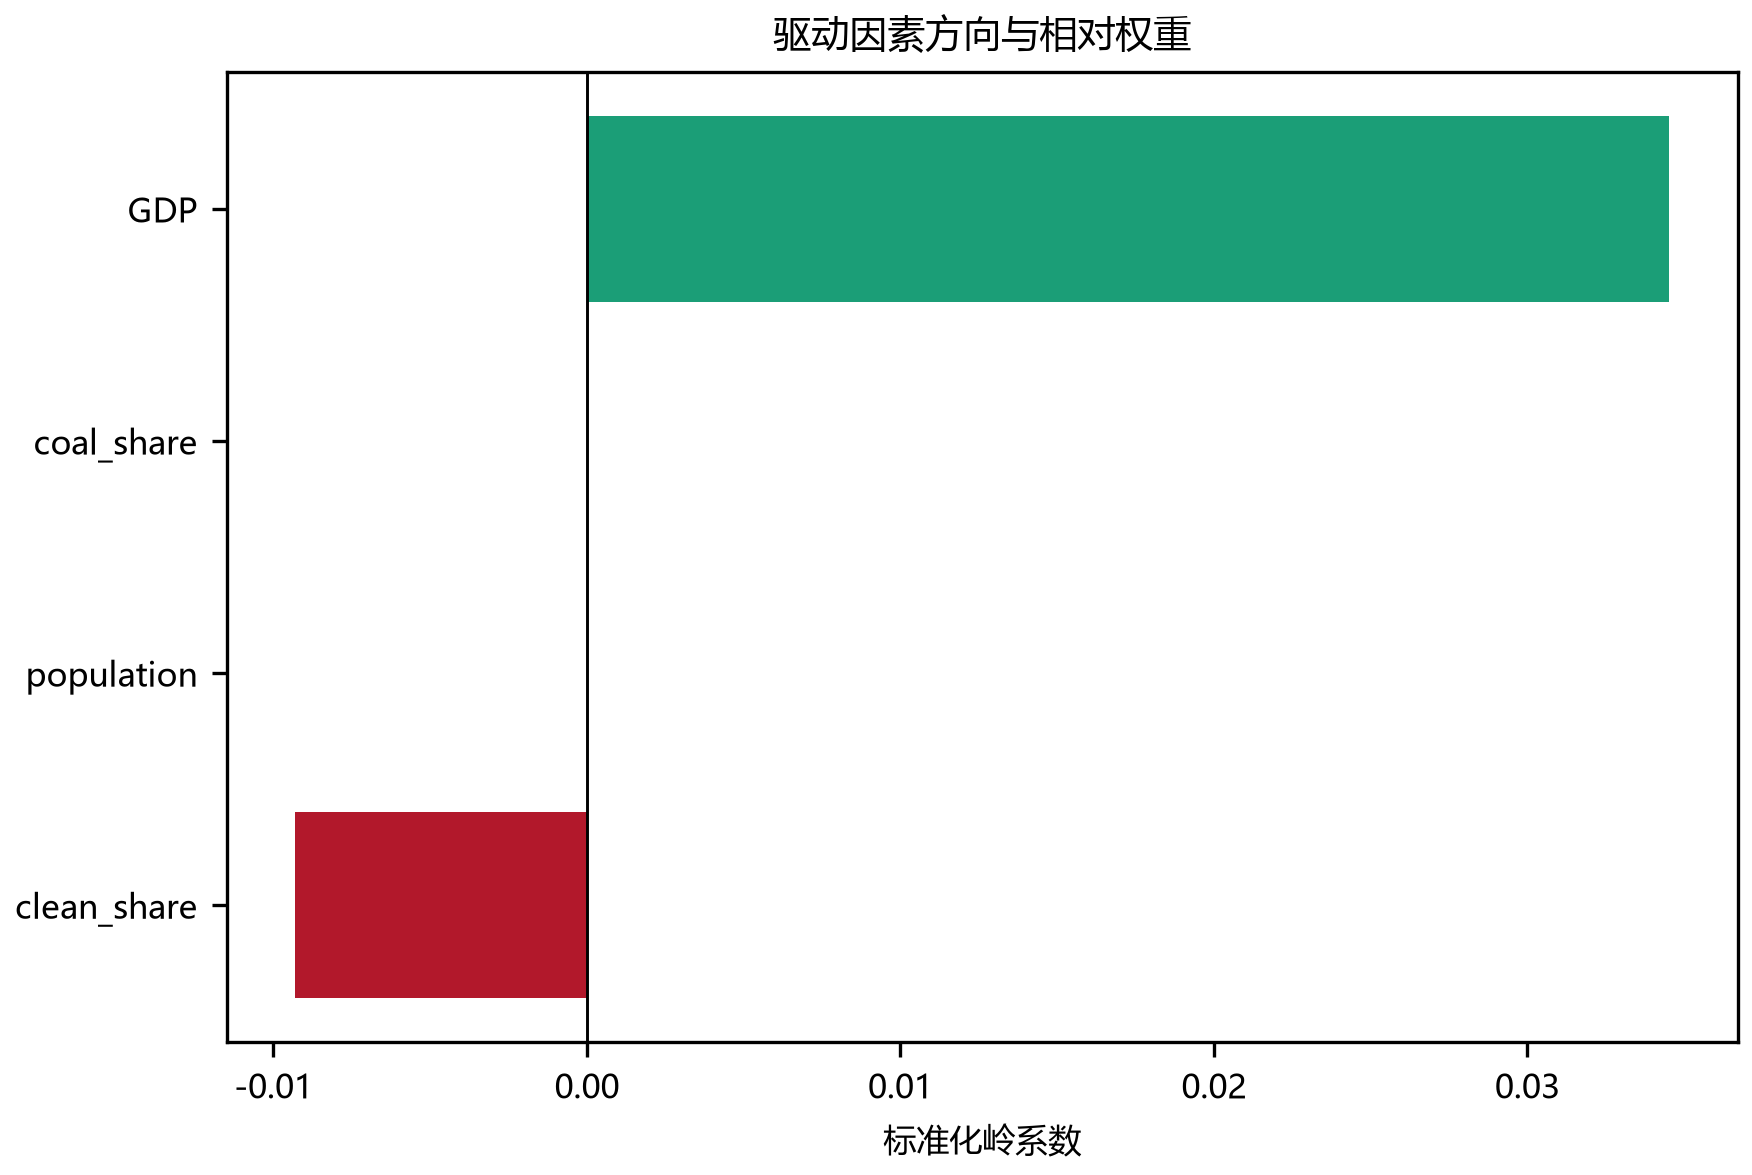
\includegraphics[width=0.80\textwidth]{figures/process_q2_coefficients.png}
\caption{驱动因素方向与相对权重}
\label{fig:q2-process}
\end{figure}

严格扩展窗口以较早年份训练、逐年预测后续年份；误差定义为
\begin{equation}
\mathrm{MAE}=\frac{1}{m}\sum_{r=1}^{m}|C_r-\widehat C_r|.
\label{eq:mae}
\end{equation}
{\sloppy 表\ref{tab:backtest}和图\ref{fig:q2-result}表明，在训练折内重新拟合标准化器后，结构模型的扩展窗口MAE为$184.397$ Mt，高于仅含时间趋势的ridge基线$157.860$ Mt。因比较窗口只有2022--2024年三个外推点，本文据此把时间趋势模型视为误差参照。结构模型只用于方向受控的解释和情景生成接口，不能把该比较夸大为长期预测精度结论。\par}

\begin{table}[H]
\centering
\caption{结构模型与时间趋势基线的回测比较}
\label{tab:backtest}
\zihao{5}
\begin{tabular}{lrr}
\toprule
指标 & STIRPAT-ridge & 时间趋势ridge\\
\midrule
扩展窗口MAE/Mt & 184.397 & 157.860\\
拟合MAE/Mt & 48.034 & --\\
拟合RMSE/Mt & 65.175 & --\\
残差标准差/Mt & 71.395 & --\\
\bottomrule
\end{tabular}
\end{table}

\begin{figure}[H]
\centering
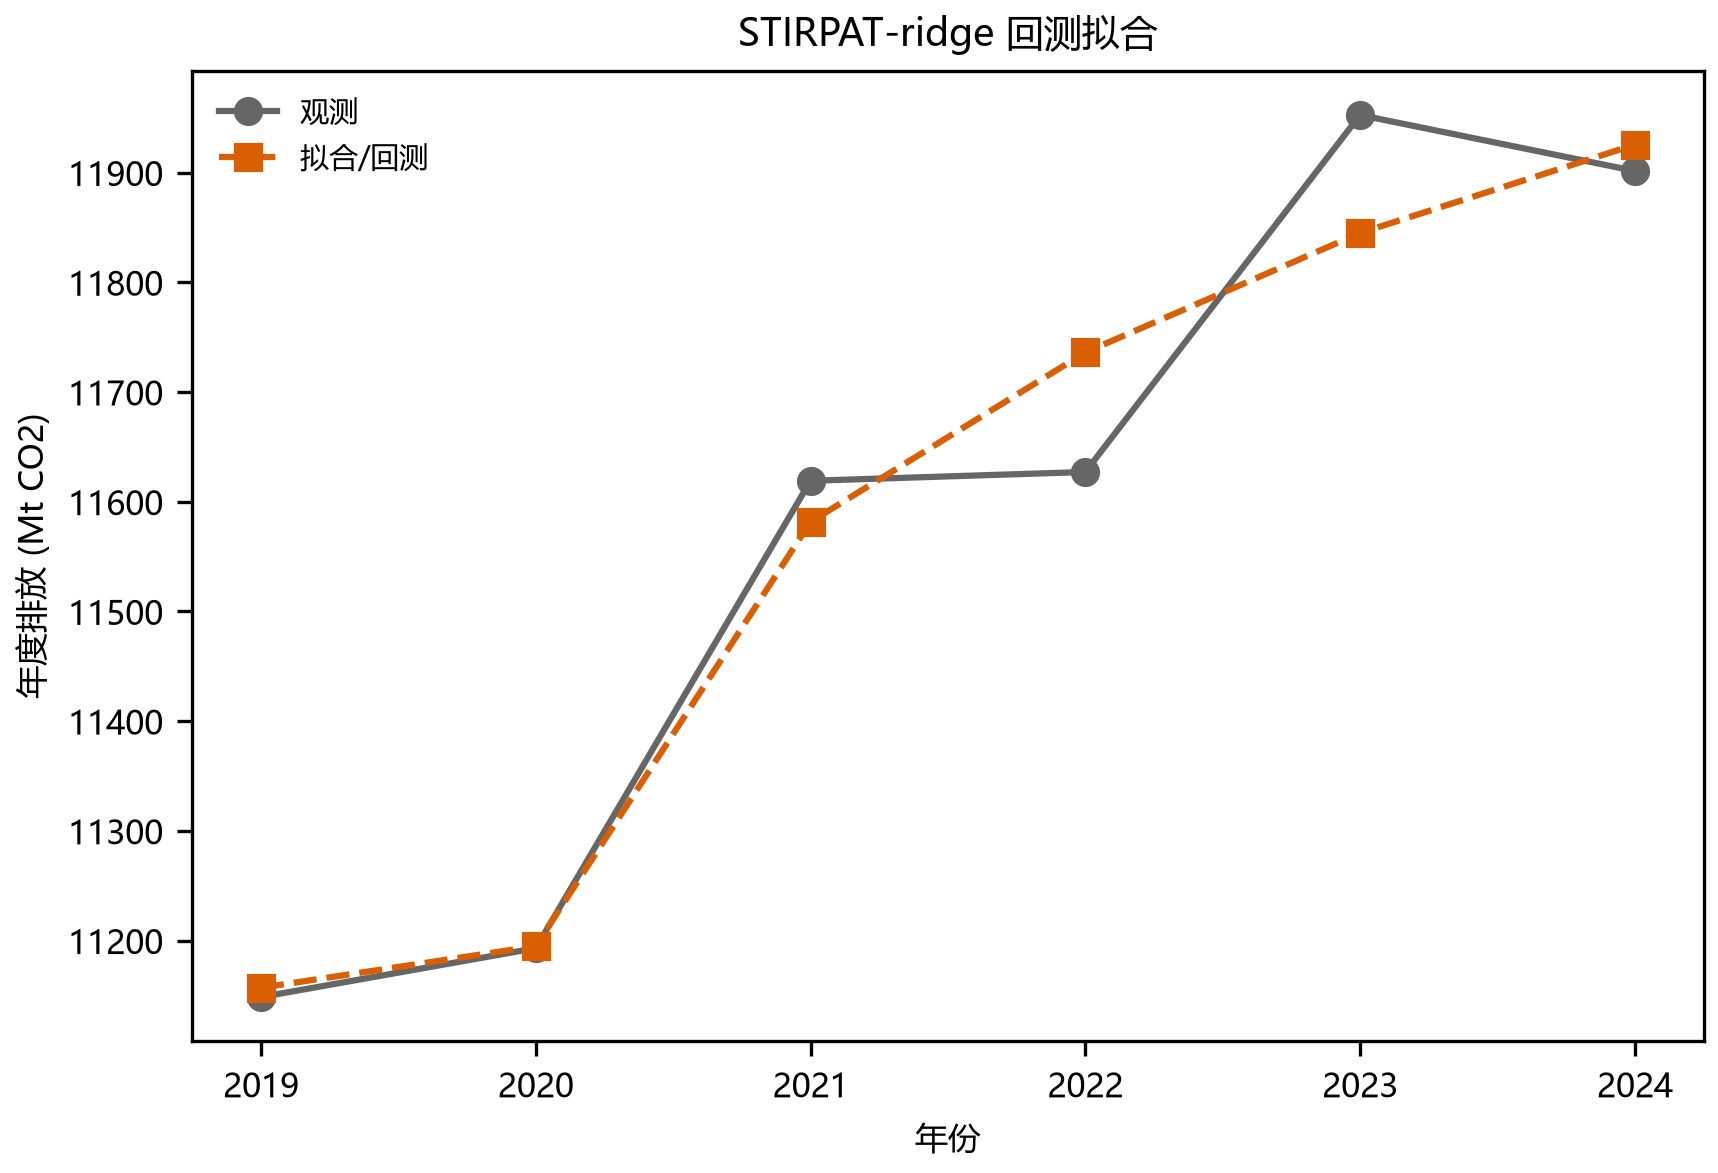
\includegraphics[width=0.86\textwidth]{figures/result_q2_backtest.png}
\caption{结构模型回测与时间趋势基线比较}
\label{fig:q2-result}
\end{figure}

\subsection{问题二结果的模型诊断}\paragraph{小样本条件下的参数解释。}
全国年度样本只有2019--2024年六个观测，因此模型的主要价值是提供一个带方向约束的结构化基线，而不是凭少量样本估计稳定的长期弹性。岭惩罚通过在残差平方和之外加入系数平方项，降低人口、GDP和能源结构变量相关时的估计波动；符号约束则把“人口、经济规模扩大不应在模型中产生负向总量贡献、清洁能源比重提高不应产生正向贡献”作为建模先验。该先验并未声称现实中不存在反例，而是为了在数据不足时避免出现难以解释的系数方向。

回测时采用扩展窗口而非随机划分。随机划分会把较晚年份的信息泄漏到较早年份，尤其不适合年度趋势预测；扩展窗口则只使用预测时点之前的数据，因而更接近真实滚动预测。MAE的比较应和基线模型一起阅读：$184.397\ \mathrm{Mt}$高于时间趋势ridge基线的$157.860\ \mathrm{Mt}$，因此模型当前不能作为优于趋势基线的点预测器；它仍可在明确符号先验和情景假设的条件下提供结构化比较，且任何未来预测都不应被赋予超出这三个回测点的精度承诺。预测部署时应保存每次训练样本、岭参数和外生变量版本，才能判断误差变化来自模型退化还是数据口径变化。

此外，标准化系数用于比较变量在样本尺度上的相对作用方向，不能直接当作原始单位下的增量效应。GDP系数为正、清洁能源比重系数为负，说明模型在样本中识别出与总量同向和反向的统计关联；这类关联可能混合了产业结构、技术进步和政策时点等未观测因素。正文因此只把系数作为情景生成的方向依据，并在局限性中明确其不具备因果识别功能。
从图\ref{fig:q2-result}可见，结构模型对2022年的扩展预测高于观测，对2023年的预测低于观测，对2024年的预测接近观测。三次预测同时用于MAE，避免只挑选误差较小年份。结构模型在部分年份的预测偏差较小，但按三个扩展窗口点的总体MAE计算，其外推误差仍高于时间趋势ridge基线，故不应宣称其具有更优的点预测精度；引入GDP和能源结构变量的价值仅限于提供方向受控的结构解释和情景接口。由于样本年份数只有6、参数含截距共5个，模型自由度有限，因此不适合报告显著性检验或进行逐变量因果归因。

为防止预测结构被误读，本文将模型使用范围限定为：全国年度总量、2019--2024年数据口径、人口/GDP/能源结构变量以及给定的情景路径。若人口统计口径、能源统计口径或部门核算范围发生结构性改变，现有系数需要重新估计；若要预测省级排放，也不能直接套用全国模型，因为省级横截面和全国时间序列的数据生成机制不同。上述边界在问题三的情景解释和问题四的政策应用中持续保留。
\subsection{预测模型的使用规范}
短样本预测的关键风险不是计算公式本身，而是把有限历史关系延伸到结构已变化的未来。本文通过三项设置降低这种风险：其一，对变量施加方向约束，避免在强共线性下出现“清洁能源比重上升导致排放上升”一类与模型设定相反的系数；其二，使用时间顺序的扩展窗口而不是随机交叉验证，避免未来年份信息泄露到训练集；其三，把趋势ridge作为纯误差基线，检验能源结构信息在外推中是否提供附加价值。

但是，上述设置并不能消除样本容量的限制。6个年度观测不足以支持复杂的高阶非线性、滞后效应或变量交互项，也不适合给出稳健的显著性水平。本文因此采用相对简单的对数结构，并通过岭正则缩小不稳定系数；模型选择的依据是可复现的预测误差与理论方向，而不是追求更高的样本内拟合度。若有新的年度观测，应按相同口径更新驱动变量、重新选择$\lambda$并复做扩展窗口比较。

对于模型输出，应区分三个层面：系数方向提示变量在给定样本中的结构关联；扩展窗口MAE衡量历史时间切分下的一步外推表现；情景预测描述外生路径条件下的可能轨迹。三者都不构成政策措施的因果效果估计。问题四据此只把系数和情景作为触发规则与监测参照，而不将其解释为某一项措施可以精确减少多少排放。
\section{问题三：多情景预测与达峰窗口判断}

\subsection{历史趋势、情景变量与约束}
图\ref{fig:q3-raw}给出全国历史年度排放趋势。三种情景从式\eqref{eq:annualize}的同一2025年化锚点出发，GDP增速按2026--2030年、2031--2035年和2036--2045年分段设置；基准、低碳和强化低碳情景的煤炭占比分别以每年0.6、1.0和1.4个百分点下降，清洁能源比重同步上升。为保证路径可行，施加
\begin{equation}
0\leq S_t^{coal}\leq1,\qquad0\leq S_t^{clean}\leq1,\qquad S_t^{coal}+S_t^{clean}\leq1.
\label{eq:scenario-constraint}
\end{equation}
图\ref{fig:q3-process}展示了三条能源结构路径。

\begin{figure}[H]
\centering
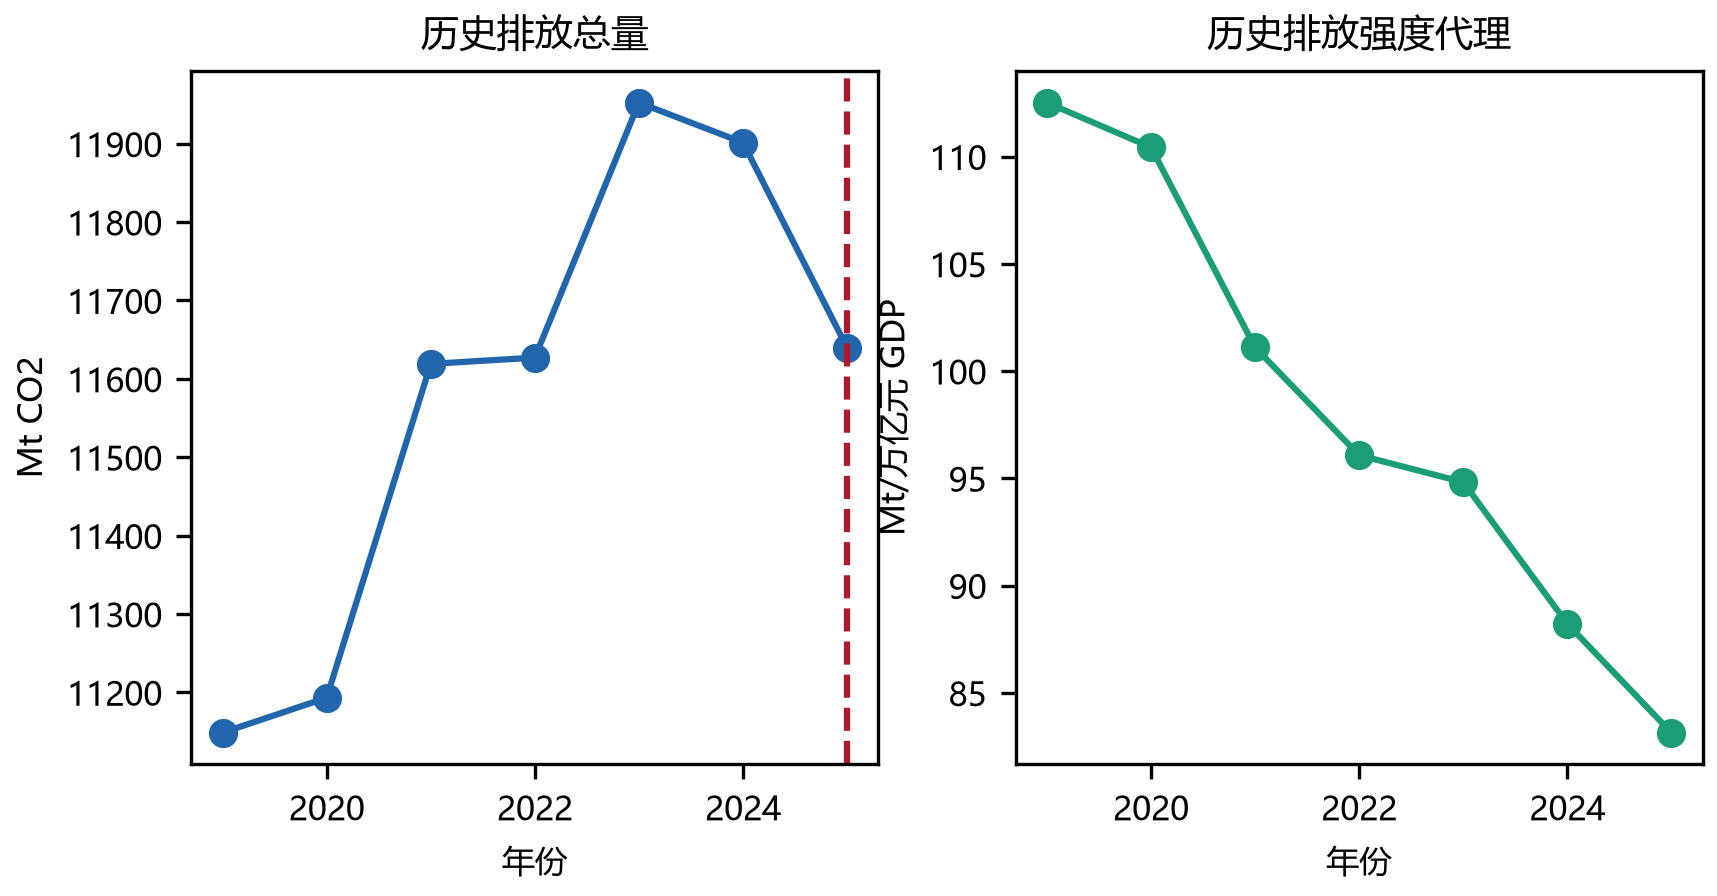
\includegraphics[width=0.86\textwidth]{figures/raw_q3_historical_trend.png}
\caption{2019--2025年全国碳排放历史趋势与2025年年化锚点}
\label{fig:q3-raw}
\end{figure}

\begin{table}[H]
\centering
\caption{三种情景的能源结构设定与约束检查}
\label{tab:scenario-path}
\zihao{5}
\begin{tabular}{lrrrr}
\toprule
情景 & 煤炭占比年降幅/百分点 & 最小煤炭占比 & 最大清洁能源比重 & 最大能源占比和\\
\midrule
基准 & 0.6 & 0.404 & 0.416 & 0.820\\
低碳 & 1.0 & 0.324 & 0.496 & 0.820\\
强化低碳 & 1.4 & 0.244 & 0.576 & 0.820\\
\bottomrule
\end{tabular}
\end{table}

\begin{figure}[H]
\centering
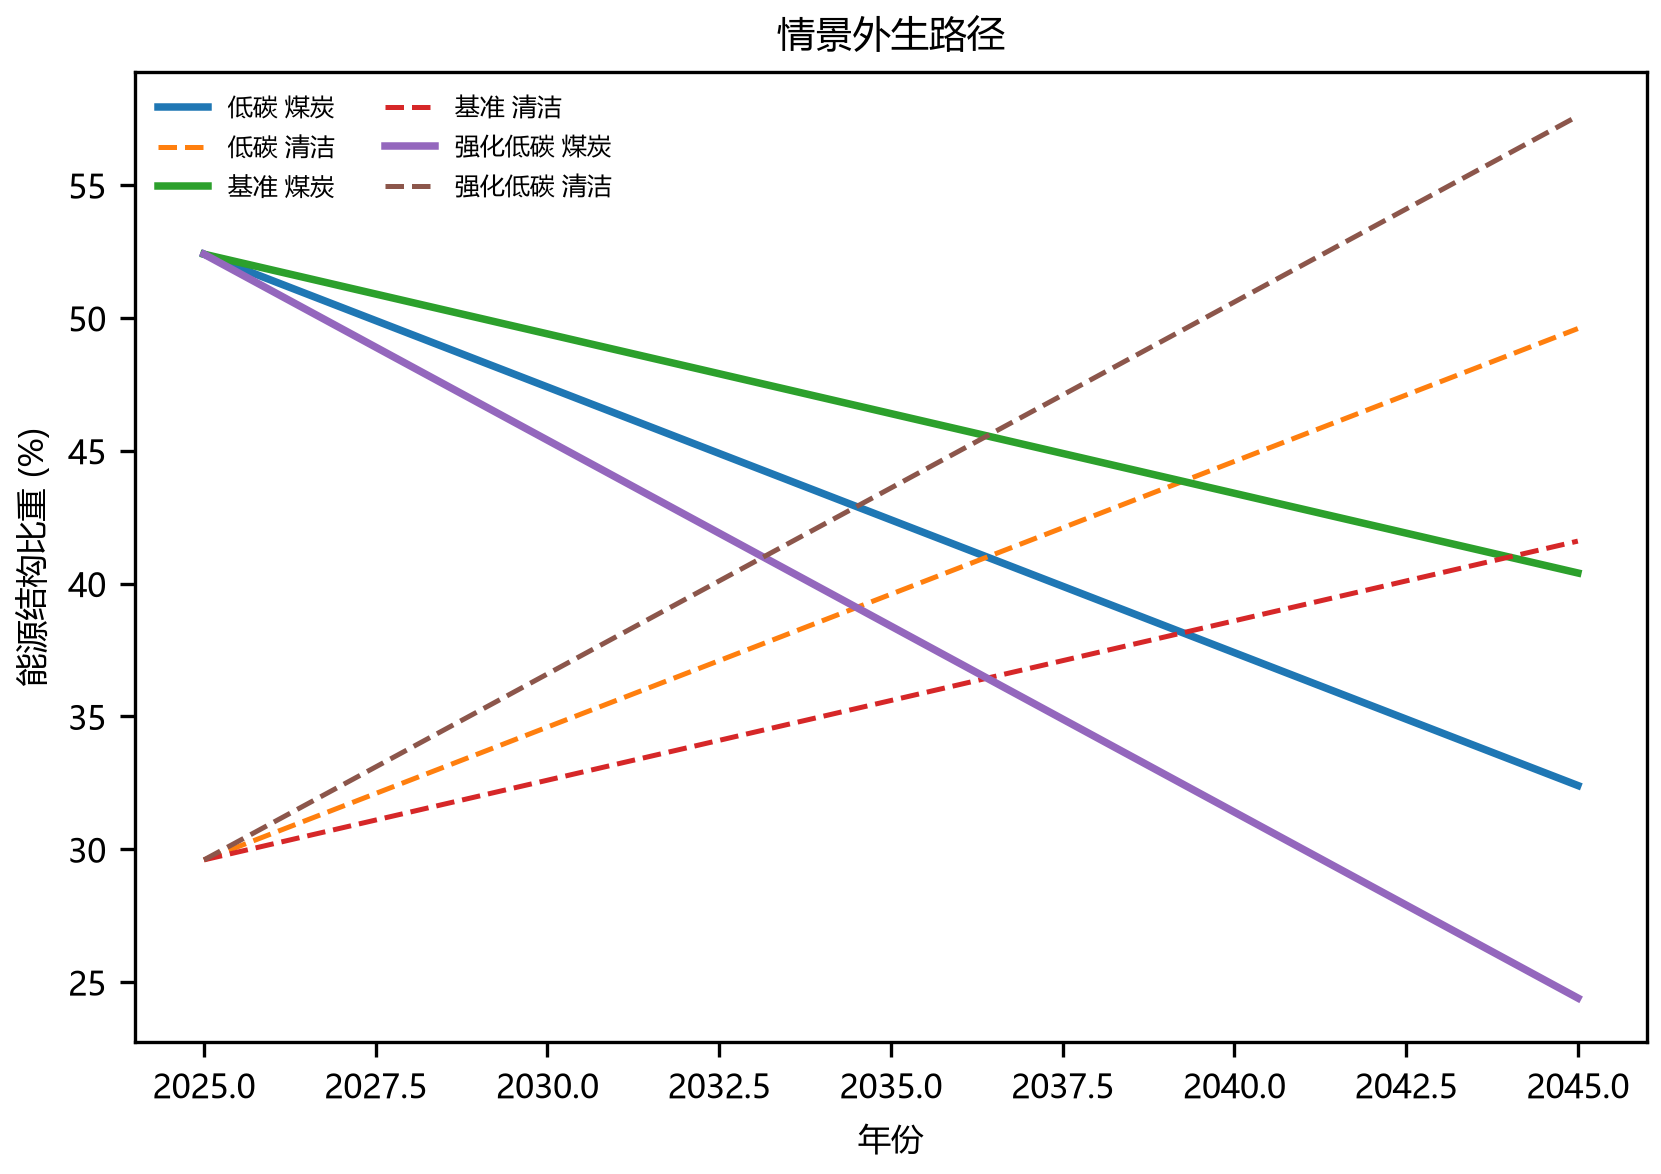
\includegraphics[width=0.86\textwidth]{figures/process_q3_scenario_paths.png}
\caption{2026--2045年三情景能源结构路径}
\label{fig:q3-process}
\end{figure}

\subsection{情景生成、校准与比较口径}
三种情景共享2025年锚点，但并不共享完全相同的外生路径。对任一情景$s$，在第$t$年按分段GDP增速更新$G_t$，人口按0.1\%年增速更新；煤炭与清洁能源比重按情景设定的年度步长推进，并保留上下界：
\begin{equation}
S_{t+1}^{coal}=\max\{0.12,S_t^{coal}-d_s^{coal}\},\qquad
S_{t+1}^{clean}=\min\{0.78,S_t^{clean}+d_s^{clean}\}.
\label{eq:scenario-path}
\end{equation}
其中$d_s^{coal}=d_s^{clean}$在基准、低碳和强化低碳情景中分别为0.006、0.010和0.014。每个年度再检验式\eqref{eq:scenario-constraint}、人口和GDP正值条件以及预测排放非负条件；这些检验输出至\texttt{问题3\_情景约束检查.csv}。

原始STIRPAT预测在2025年可能与年化锚点存在有限差异，因此先计算共同校准因子0.967299，使三条路径在2025年从同一个$11639.658$ Mt起点出发。校准只改变共同尺度，不改变不同情景之间由外生路径决定的相对排序。这样，情景比较关注2026年后的GDP、煤炭与清洁能源变化，而不会把起点统计口径误差混入政策差异。

总量和强度必须同时比较。总量反映大气排放压力，强度反映经济活动的排放效率；当不同情景的GDP增长路径不同时，两者的排序可以不同。表\ref{tab:scenario}中2045年低碳情景的强度低于强化低碳情景，但其总量仍高于强化低碳情景，正是因为两项指标共同受分母GDP和分子排放路径影响。故本文不把任一单一指标作为情景优劣的唯一结论，而是把它们并列作为问题四的阶段监测对象。
\subsection{总量与强度预测}\paragraph{情景路径的内部一致性检查。}
三种情景并不是分别拟合三套模型，而是在同一组模型参数下改变外生变量的演化路径。这样处理能够把情景差异集中归因于人口、GDP、煤炭占比和清洁能源比重的设定，避免因重复估计而引入额外的参数差异。基准情景保持相对平缓的能源转型速度，低碳情景和强化低碳情景逐步加大煤炭占比下降幅度，并同步设置清洁能源比重的改善路径。由于外生路径属于假设，情景名称表示政策强度层级，不表示官方规划或必然发生的未来。

在计算流程中，先生成2026--2045年的年度外生变量，再将其代入问题二的拟合关系，最后依据人口或GDP路径计算排放强度。每一条路径都要满足非负性、比例变量位于合理区间以及年度变化方向不反转等基本约束。若某条路径出现煤炭占比低于零、清洁能源比重超过100\%或总量排序交叉，代码应在输出阶段报错，而不能通过图形平滑掩盖。当前结果中强化低碳$<$低碳$<$基准的排序在整个预测窗口内保持一致，说明设定的路径具有内部一致性，但不代表不同情景之间的差异已达到统计显著。

排放强度与排放总量承担不同的判断功能。总量用于识别全国碳预算压力，强度用于观察经济增长背景下单位产出排放是否下降；在GDP持续增长时，总量可能暂时上升而强度下降，两者并不矛盾。因而政策评估不能只看总量曲线，也应同时跟踪强度、煤炭占比和部门构成，并把年度实际值与同一情景的预测值进行滚动比较。
对每条外生路径代入式\eqref{eq:stirpat}并以2025年锚点校准，得到2026--2045年的排放预测。排放强度定义为
\begin{equation}
I_t^{GDP}=\frac{C_t}{G_t},
\label{eq:intensity}
\end{equation}
其单位为Mt/(万亿元 GDP)。每个情景包含1行2025年锚点和20行预测，共输出63行；所有预测行均通过GDP、人口、能源占比和排放非负性检查。关键年份结果见表\ref{tab:scenario}，总量及强度的完整走势见图\ref{fig:q3-result}。

\begin{table}[H]
\centering
\caption{三种情景的关键年份预测结果}
\label{tab:scenario}
\zihao{5}
\begin{tabular}{llrrr}
\toprule
情景 & 年份 & 总量/Mt & 强度/(Mt/万亿元 GDP) & 煤炭占比/(\%)\\
\midrule
基准 & 2025 & 11639.658 & 82.170 & 52.4\\
基准 & 2030 & 12248.657 & 69.387 & 49.4\\
基准 & 2045 & 13864.762 & 45.765 & 40.4\\
低碳 & 2045 & 13437.482 & 44.355 & 32.4\\
强化低碳 & 2045 & 12890.561 & 44.652 & 24.4\\
\bottomrule
\end{tabular}
\end{table}

在2026--2045年内，三种情景总量始终保持强化低碳$<$低碳$<$基准。2045年总量分别为12890.561、13437.482和13864.762 Mt CO$_2$；2045年强度排序为低碳$<$强化低碳$<$基准。这一差异表明总量与强度共同受GDP路径和能源结构影响，不能只用单一指标评估情景表现。由于三条路径的窗口最大值均位于2045年边界，本研究的可支持判断是“预测窗口内未见达峰，峰值可能在2045年以后”，而不是把2045年直接称为已达峰。

\begin{figure}[H]
\centering
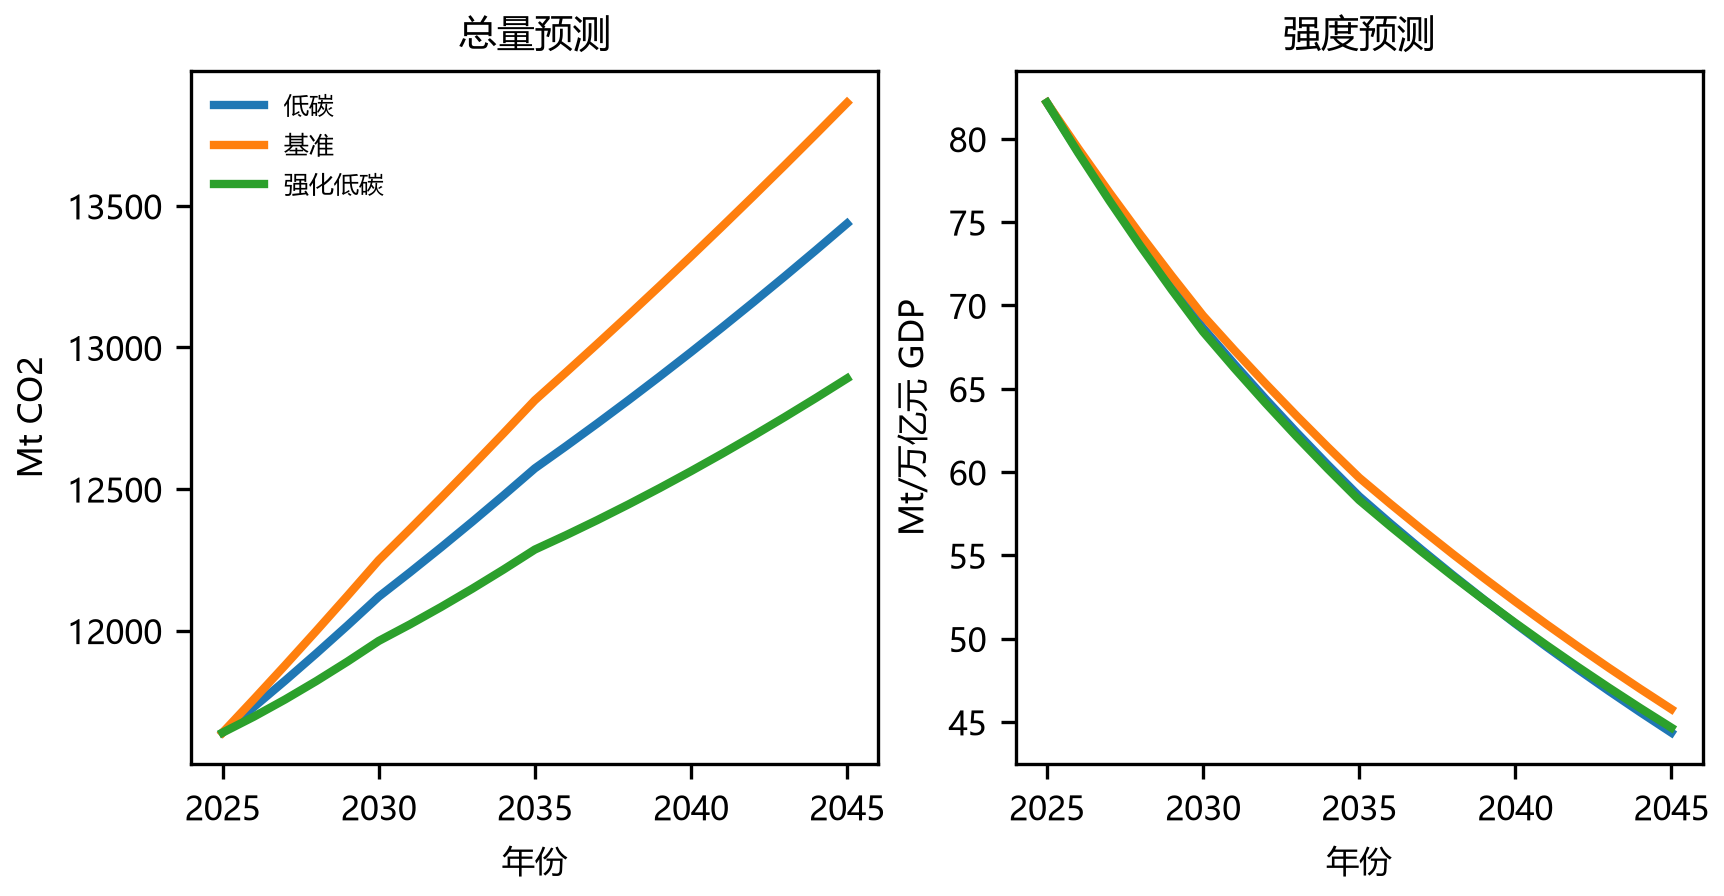
\includegraphics[width=0.88\textwidth]{figures/result_q3_forecast.png}
\caption{2026--2045年三情景排放总量与强度预测}
\label{fig:q3-result}
\end{figure}

\subsection{达峰判断的边界与风险提示}
达峰判断采用预测区间内总量最大值的定义。若最大值出现在区间内部，才可以在给定情景内报告该年为窗口峰值；若最大值出现在右端点2045年，则只能说明模型在观察窗口内仍保持上升，无法判断2045年以后是否继续上升、转平或下降。三种情景均属于后一种情况，因此本文避免使用“2045年实现碳达峰”等超出数据支持范围的表述。

情景间的差异也应按条件解释。低碳和强化低碳路径在煤炭占比下降、清洁能源比重上升及GDP增长假设上不同，因此总量差异同时包含结构调整和经济规模路径的共同作用。若未来GDP增长、人口变化或能源技术进展偏离本文设定，预测轨迹会随之改变。表\ref{tab:scenario-path}列出的最小煤炭占比、最大清洁能源比重和能源占比和，保证的是路径数学可行性，不是未来实际实现的概率。

为使风险提示能够落到年度数据上，建议每年将观测到的GDP、煤炭比重、清洁能源比重和全国总量与相应情景路径逐项比较。若总量高于路径上界或能源结构改善慢于路径设定，应先检查数据口径和异常部门，再评估是否需要加强总量控制、能效改造或能源替代；若总量低于路径但强度改善不足，则应进一步观察GDP波动是否改变了分母效应。这样的比较比单纯追踪“是否到达某个峰值年份”更适合滚动决策。
\section{问题四：差异化减排建议与监测闭环}

\subsection{可复现的政策映射规则}
问题四以问题一的类别和重点治理标记、全国部门累计排放与问题三的情景预测为输入，不额外估计无法验证的政策弹性。对第$i$个省份，构造五个二元工具标识：
\begin{equation}
\begin{aligned}
z_{i}^{T}&=\mathbb{I}\{\text{priority}_i=\text{重点治理}\},&
z_{i}^{E}&=\mathbb{I}\{EI_i\geq\operatorname{median}(EI)\},\\
z_{i}^{C}&=\mathbb{I}\{S_{i}^{coal}\geq\operatorname{median}(S^{coal})\},&
z_{i}^{M}&=\mathbb{I}\{L_i\geq\operatorname{median}(L)\},\\
z_{i}^{D}&=\mathbb{I}\{E_i\geq\operatorname{median}(E),\ S_{i}^{coal}<\operatorname{median}(S^{coal})\},
\end{aligned}
\label{eq:policy-map}
\end{equation}
其中$T,E,C,M,D$依次对应总量控制、能效改造、煤炭替代、市场机制和需求侧治理，$L_i$为经济联系指数。阈值由30省样本的中位数计算：$EI$为0.9576 t/(万元 GDP)、煤炭排放占比为75.5658\%、经济联系指数为0.0220、排放规模为303.1388 Mt。该规则及所有省级标识写入\texttt{问题4\_省级政策映射.csv}，从而使图表和政策对象均可由结果文件复算。

部门累计排放的排序见图\ref{fig:q4-raw}。工业和电力部门的累计排放占比分别为46.20\%和39.08\%，是部门侧优先关注对象。类别--工具覆盖率由上述省级规则聚合得到，见图\ref{fig:q4-process}和表\ref{tab:q4-policy}。

\begin{figure}[H]
\centering
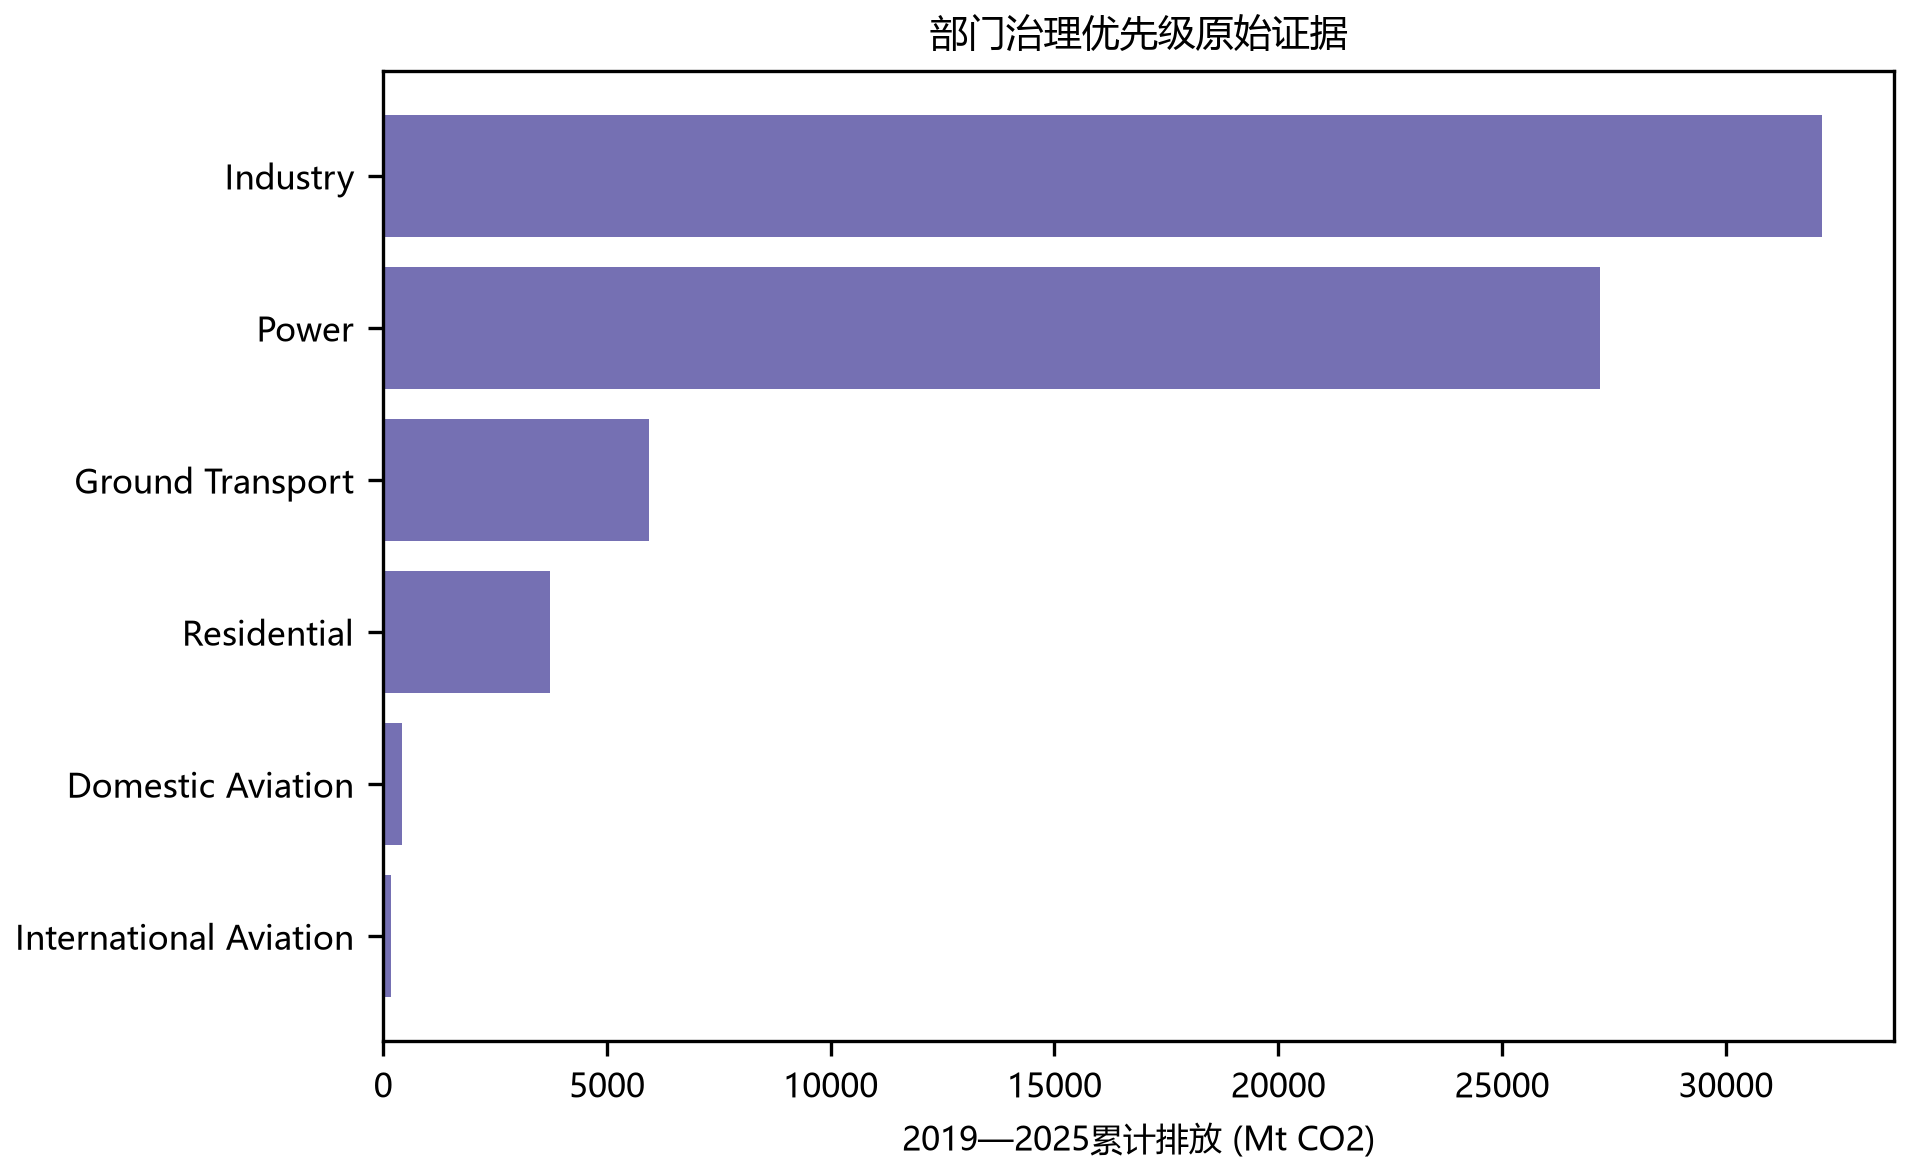
\includegraphics[width=0.86\textwidth]{figures/raw_q4_sector_share.png}
\caption{2019--2025年全国分部门累计排放及治理优先级}
\label{fig:q4-raw}
\end{figure}

\begin{figure}[H]
\centering
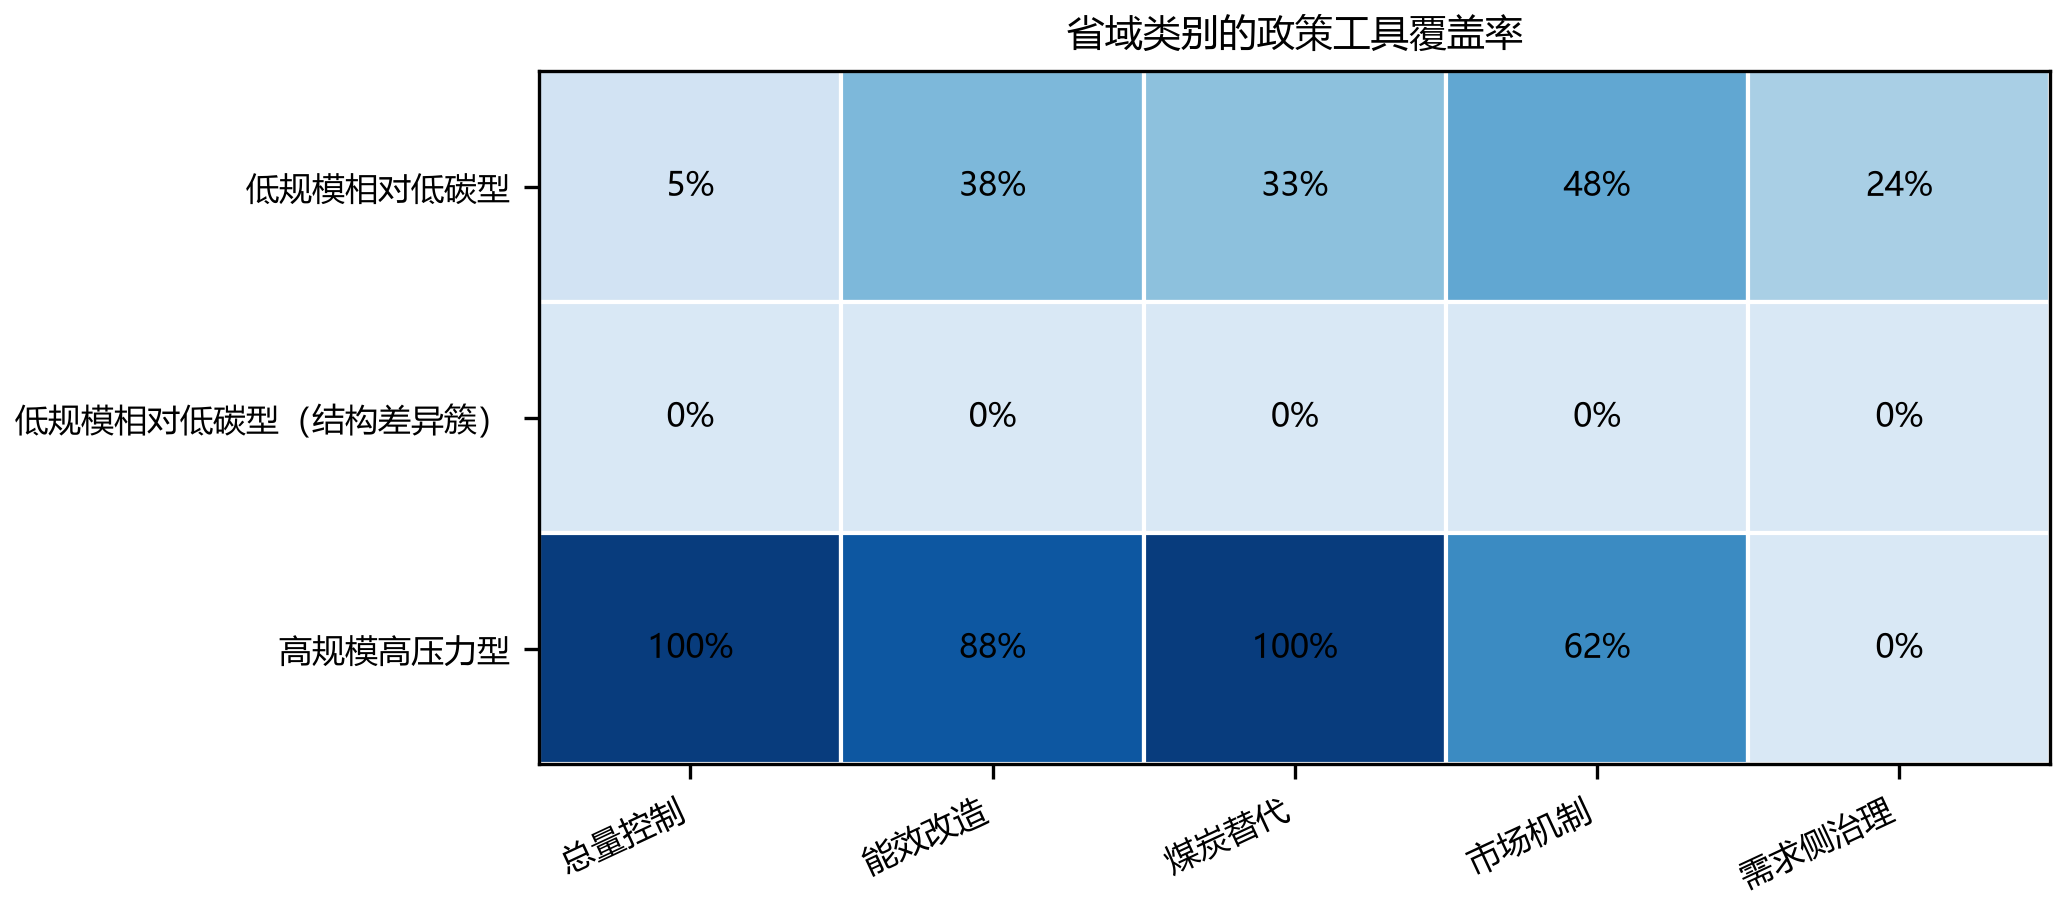
\includegraphics[width=0.90\textwidth]{figures/process_q4_policy_matrix.png}
\caption{按省级规则计算的类别政策工具覆盖率}
\label{fig:q4-process}
\end{figure}

\subsection{分类型、分部门建议}
表\ref{tab:q4-policy}中的百分比表示同类省份中满足相应触发条件的比例，而非政策实施后的减排比例。高规模高压力型的8个省份中，100\%触发总量控制和煤炭替代，87.5\%触发能效改造，62.5\%触发市场机制；因此该类地区应优先将重点行业碳预算、设备更新与煤炭替代组合实施。低规模相对低碳型的21个省份中，38.1\%触发能效改造、33.3\%触发煤炭替代、47.6\%触发市场机制，说明同一类别内部仍需按省级指标选择工具。北京作为结构差异簇未触发样本中位数规则，需结合服务业、交通和建筑终端特征进行个案复核，而不是直接套用高排放地区措施。

\begin{table}[H]
\centering
\caption{按省级规则计算的类别政策工具覆盖率}
\label{tab:q4-policy}
\zihao{5}
\resizebox{\textwidth}{!}{%
\begin{tabular}{lrrrrrr}
\toprule
类别 & 省份数 & 总量控制/(\%) & 能效改造/(\%) & 煤炭替代/(\%) & 市场机制/(\%) & 需求侧治理/(\%)\\
\midrule
高规模高压力型 & 8 & 100.0 & 87.5 & 100.0 & 62.5 & 0.0\\
低规模相对低碳型 & 21 & 4.8 & 38.1 & 33.3 & 47.6 & 23.8\\
低规模相对低碳型（结构差异簇） & 1 & 0.0 & 0.0 & 0.0 & 0.0 & 0.0\\
\bottomrule
\end{tabular}}
\end{table}

\subsection{分阶段情景指标与年度复盘}
问题三的三条情景为阶段推进提供可监测的参照，而非强制指标。表\ref{tab:q4-phase}给出各阶段末的强度指数，其中指数以情景内2025年强度为100。到2045年，基准、低碳和强化低碳情景的强度指数分别为55.70、53.98和54.34，对应强度降幅44.30\%、46.02\%和45.66\%。图\ref{fig:q4-result}由这9条阶段结果直接绘制，替代了此前的人工目标序列。

\begin{table}[H]
\centering
\caption{三情景阶段末排放强度指数与能源结构指标}
\label{tab:q4-phase}
\zihao{5}
\resizebox{\textwidth}{!}{%
\begin{tabular}{llrrrr}
\toprule
情景 & 阶段末 & 强度指数(2025=100) & 强度降幅/(\%) & 煤炭占比/(\%) & 清洁能源比重/(\%)\\
\midrule
基准 & 2030 & 84.44 & 15.56 & 49.4 & 32.6\\
基准 & 2035 & 72.61 & 27.39 & 46.4 & 35.6\\
基准 & 2045 & 55.70 & 44.30 & 40.4 & 41.6\\
低碳 & 2030 & 83.55 & 16.45 & 47.4 & 34.6\\
低碳 & 2035 & 71.24 & 28.76 & 42.4 & 39.6\\
低碳 & 2045 & 53.98 & 46.02 & 32.4 & 49.6\\
强化低碳 & 2030 & 83.27 & 16.73 & 45.4 & 36.6\\
强化低碳 & 2035 & 70.97 & 29.03 & 38.4 & 43.6\\
强化低碳 & 2045 & 54.34 & 45.66 & 24.4 & 57.6\\
\bottomrule
\end{tabular}}
\end{table}

年度复盘至少核对排放总量、单位GDP排放、煤炭与清洁能源比重、部门排放和数据质量五类指标。2026--2030年优先夯实核算口径、重点行业节能改造和能效提升；2031--2035年依据阶段指数提升清洁能源替代与系统调节能力；2036--2045年依据总量、强度和能源结构偏离程度滚动更新措施。若监测结果偏离表\ref{tab:q4-phase}的对应情景路径，应先复核数据口径、产业变化和能源结构，再调整政策工具。

\begin{figure}[H]
\centering
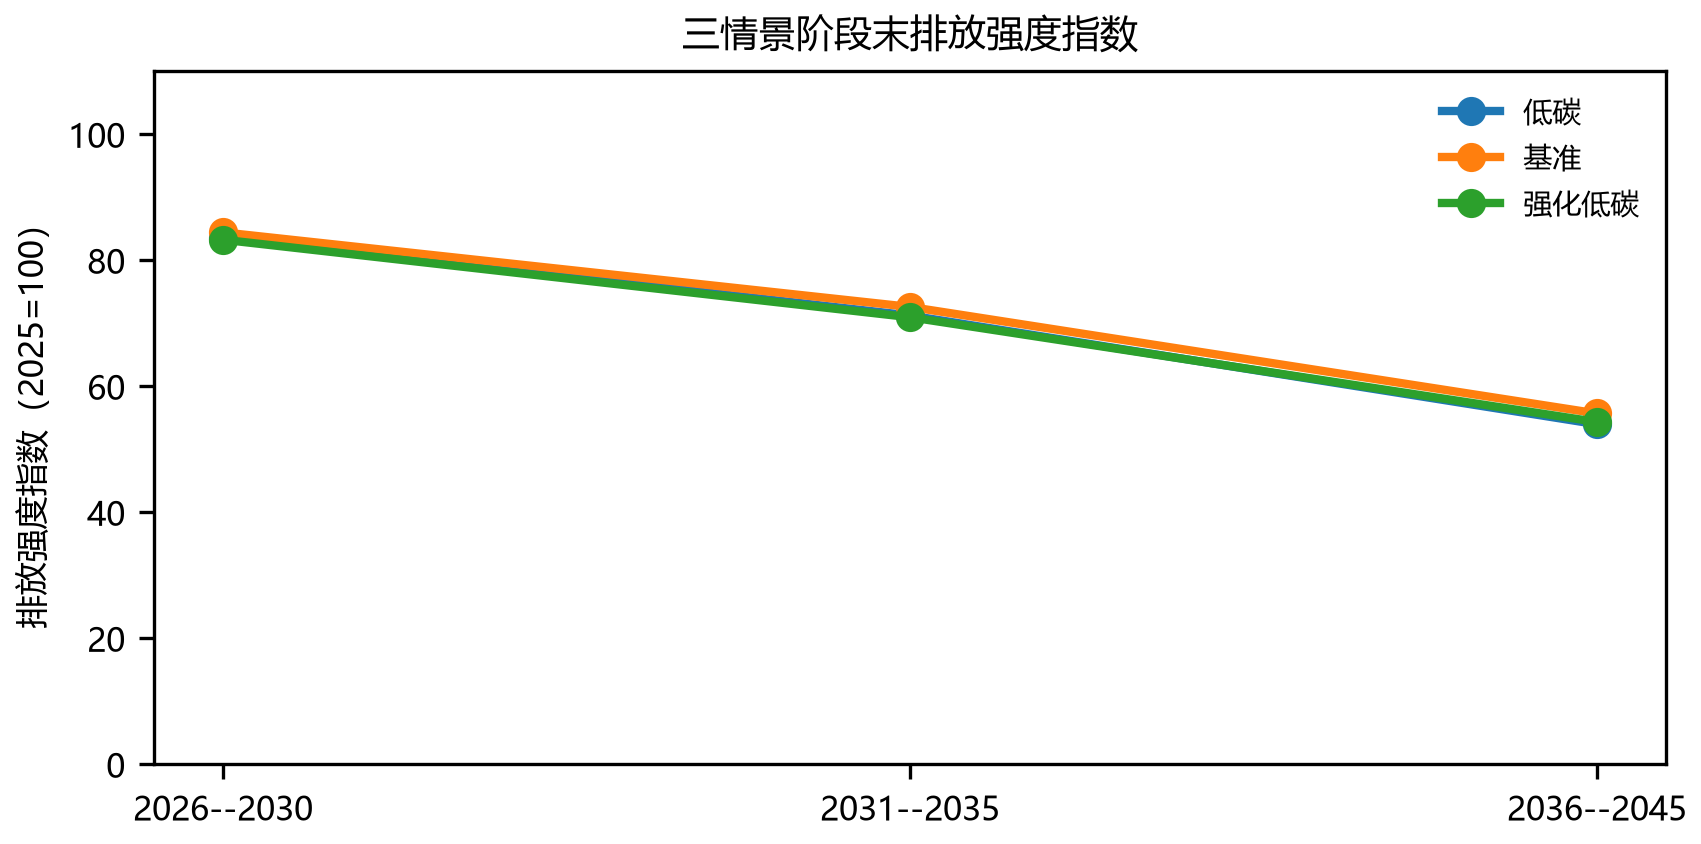
\includegraphics[width=0.86\textwidth]{figures/result_q4_roadmap.png}
\caption{由情景预测结果计算的三情景阶段末强度指数}
\label{fig:q4-result}
\end{figure}
\subsection{政策结果的聚合与使用边界}
问题四的政策图不是把类别名称直接翻译为措施，而是先对每个省份按式\eqref{eq:policy-map}计算五个工具标识，再按类别求各标识的平均值。若类别$g$中有$n_g$个省份，则某工具$r$的覆盖率为
\begin{equation}
R_{g,r}=\frac{100}{n_g}\sum_{i\in g}z_i^{r}.
\label{eq:policy-coverage}
\end{equation}
因此，表\ref{tab:q4-policy}的100\%表示该类别的所有省份满足该项触发规则，4.8\%表示21个省份中约有1个满足规则；它既不是减排承诺，也不是政策成效估计。这个定义使“类别--工具覆盖率”可以从\texttt{问题4\_省级政策映射.csv}逐行重新聚合，并由\texttt{问题4\_类别政策覆盖率.csv}直接核验。

部门优先级同样使用实际累计排放而非主观排序。工业与电力合计占2019--2025年六类部门累计排放的85.27\%，故工业能效、过程排放控制、电力低碳替代和系统调节是部门层面的优先方向；地面交通占8.52\%，住宅占5.37\%，可在需求侧治理中分别通过公共交通、电动化、建筑节能和分时价格工具跟踪。国际和国内航空在本数据口径中占比较低，但仍应保持独立统计，避免与国内部门总量重复计量。

阶段指标不是预先设定的行政目标。图\ref{fig:q4-result}和表\ref{tab:q4-phase}使用问题三的9个阶段末预测值，分别展示三情景在2030、2035和2045年的强度指数、煤炭占比和清洁能源比重。实际年度监测若偏离相应情景，可以先判断偏离来自总量、GDP、能源结构还是部门排放，再回到省级工具规则调整治理重点；这一过程形成“数据更新--规则计算--措施调整--下一期核验”的滚动闭环。
\subsection{数据治理与政策闭环的实施口径}\paragraph{政策执行、评估与回滚机制。}
政策闭环需要把“建议”转化为可检查的年度动作。执行层面可先按省级政策映射表建立责任清单，再将总量控制、能效改造、煤炭替代、市场机制和需求侧治理分别对应到重点行业、能源设施、交易机制和终端用能环节。评估层面不以单一年度总量作唯一依据，而是同时检查总量、排放强度、煤炭占比、部门排放份额和数据完整率；当实际值偏离情景路径时，先核对统计口径和数据延迟，再判断是否需要调整政策强度。

对于跨年度的指标，应使用同一口径计算同比变化，避免因统计范围、排放因子或部门分类变更造成虚假波动。若输入文件新增年份，程序应重新执行附件1的总量核验、年化处理和部门汇总，并保存新旧版本的哈希。若某项指标缺失，则应标注为待核验，而不宜用零值代替。只有在数据质量检查通过后，才将实际值写入下一轮模型训练和政策复盘表。

滚动机制可按“年度更新、三年复盘、重大口径变更即时重估”执行。年度更新用于修正短期路径，三年复盘用于重新检验聚类稳定性、回测误差和政策工具覆盖率；当能源统计制度或部门定义发生重大变化时，应重新建立可比序列。该流程不需要预先承诺某项政策必然有效，而是把模型作为监测和调整工具，使政策建议具有可撤回、可修正的操作空间。
政策闭环要能够在数据更新后被重复执行，因而首先需要固定数据口径。全国日频数据应持续保留\texttt{Total}、五个国内部门与国际航空的对应关系；若部门分类调整，应在历史序列中记录断点而非直接拼接。省级清单应保持排放范围、GDP价格口径和人口口径的一致，并在缺失省份或修订年份出现时重新计算分位数阈值。只有当输入口径一致，式\eqref{eq:priority}和式\eqref{eq:policy-map}的触发结果才具有跨年度可比性。

其次，监测频率应与指标性质相匹配。全国部门排放和能源结构可按月度或季度跟踪，用于尽早识别路径偏离；GDP、人口和省级清单通常按年度更新，用于重新计算强度、类别和工具覆盖率。对每一次更新，应同时保存输入版本、计算日期、随机种子、代码哈希和结果哈希。项目中的\texttt{复现清单.json}已经提供了这一记录格式，后续数据更新可以沿用同一结构，从而区分“数据变化导致的结果变化”和“代码变化导致的结果变化”。

再次，政策工具不能只记录是否触发，还应建立措施执行与结果反馈的链条。对总量控制工具，可记录重点行业碳预算覆盖率和实际排放；对能效改造工具，可记录单位工业增加值能耗、设备更新投资和过程排放占比；对煤炭替代工具，可记录煤炭占比、清洁能源消纳、储能与需求响应；对市场机制，可记录履约率和核算偏差；对需求侧治理，可记录交通排放、建筑能耗和峰谷负荷差。这样，问题四的二元规则负责识别“优先关注什么”，监测指标负责判断“措施是否产生预期方向的变化”。

最后，结构差异簇和低覆盖率工具不能被误解为不采取行动。它们表示在本文的中位数规则下没有触发相应的通用条件。对于北京这类单独簇，建议以服务业、交通、建筑和终端用能数据补充个案分析；对于其他低覆盖率工具，也应结合地方产业、能源供应和政策成本作二次判断。本文提供的是可复现的筛选框架，不替代地方部门的详细工程评估。
\subsection{跨问题证据链与结果解释}
本文四个问题之间存在明确但有限的递进关系。问题一只使用2022年省级清单，输出空间集聚证据、类别与重点治理标记；它不直接预测全国总量。问题二只使用2019--2024年全国年度序列，输出方向受控的结构模型和扩展窗口误差；它不以省级类别作为回归样本。问题三将问题二模型代入外生路径，并以2025年化值校准，输出三情景年度总量、强度和路径可行性。问题四最后同时使用问题一的省级标识、全国部门累计排放和问题三的阶段指标，输出工具覆盖率和监测参照。这样的分工避免将横截面分类误当作时间序列的因果变量，也避免将情景参数直接写成地方政策效果。

每个核心主张均有至少一种直接证据。空间集聚结论由表\ref{tab:moran}的观测Moran $I$与999次置换$p$值支撑，分类数由表\ref{tab:silhouette}及\texttt{问题1\_聚类决策.csv}支撑，省域类型由表\ref{tab:cluster}和图\ref{fig:q1-result}支撑。结构模型与趋势基线的误差比较由表\ref{tab:backtest}和图\ref{fig:q2-result}支撑，且表明当前结构模型的扩展窗口误差更高；不对系数作因果解释的限制来自样本数、约束边界和时间顺序验证。情景排序、2045年数值和未见达峰判断由表\ref{tab:scenario}、图\ref{fig:q3-result}以及右端点峰值规则支撑。问题四的部门优先级、工具覆盖率和阶段指数则分别可在\texttt{问题4\_部门优先级.csv}、\texttt{问题4\_类别政策覆盖率.csv}和\texttt{问题4\_阶段情景指标.csv}中逐项核对。

这种证据链也规定了结论可以说到什么程度。例如，“显著空间集聚”只适用于表\ref{tab:moran}中通过5\%置换检验的指标；“模型误差比较”只适用于既定三个扩展窗口与时间趋势基线的比较，且不延伸为长期精度承诺；“强化低碳总量较低”只适用于给定外生路径的2026--2045年窗口；“某类地区优先采用某工具”只表示规则触发程度较高，而不等价于已估计该工具的减排效应。通过将每个结论限制在对应数据、模型和时间范围内，本文尽量避免由统计描述推到因果判断，或由情景模拟推到政策承诺。
\section{模型检验、评价与适用边界}

\subsection{结果核验与可复现性}
本文的关键数值均由项目代码实际运行获得：输入数据17255行、空间Moran检验采用999次固定种子置换、聚类数$k=3$、岭参数0.0429449、情景预测63行。2025年年化、问题二扩展窗口回测和问题三路径约束分别由式\eqref{eq:annualize}、表\ref{tab:backtest}和表\ref{tab:scenario-path}支撑；图\ref{fig:q1-result}、图\ref{fig:q2-result}、图\ref{fig:q3-result}和图\ref{fig:q4-result}分别对应四个问题的正式结果图。执行环境、随机种子、输入哈希和复现命令记录在附录A中。

\subsection{模型优点}\paragraph{模型检验的补充说明。}
四个问题之间采用“横截面画像--时间序列解释--情景外推--政策映射”的顺序，既利用了不同附件的优势，也避免把省级数据强行拼接到全国年度模型中。横截面模型主要回答地区之间如何不同，时间序列模型主要回答全国排放与驱动变量如何共同变化，情景模型回答给定外生路径下的可能范围，政策映射则回答如何把统计结果转化为分层任务。四个环节的统计对象和时间尺度不同，因此不能用某一环节的误差指标替代另一环节的验证。

从复现角度看，论文中的关键结果应满足三项条件：第一，结果表中的数值能够由固定输入和随机种子重新生成；第二，图表只读取结果文件，不在绘图脚本中另行写入不可追溯常量；第三，正文主张能够回指公式、表格、图或复现清单。当前项目将问题四的省级政策映射、类别覆盖率、阶段指标和部门优先级单独保存，因而政策建议仍可在不改动正文的情况下随数据版本更新。若更新后的结果改变了排序或覆盖率，正文应同步重写，而不能只替换图片。
\begin{enumerate}[label=(\arabic*)]
\item 先进行\texttt{Total}口径核验并区分全国时间序列和省级横截面，避免把不同来源、不同层级的数据重复计量。
\item 对空间差异同时报告Moran检验、轮廓系数和分类解释，并以轮廓系数最大规则确定$k=3$，使分类决策可由结果表复核。
\item STIRPAT-ridge将能源结构方向约束纳入估计，并以扩展窗口MAE与时间趋势基线比较，避免仅报告样本内拟合误差。
\item 政策建议由省域类别、部门结构、情景差异和监测指标逐层映射，能够支持年度滚动复盘。
\end{enumerate}

\subsection{局限性与改进方向}
\begin{enumerate}[label=(\arabic*)]
\item 全国驱动模型只有6个年度观测，参数不确定性较大；模型系数只能做结构性解释，不能作为因果效应或精确长期点预测。
\item 省级样本不含西藏，海南采用桥接空间关系；全局Moran检验不能替代基于真实经济联系、能源流或电网拓扑的空间网络分析。
\item 外生GDP和能源结构路径是情景假设而非官方规划，经验残差带也不是正式置信区间；2045年边界最大值不能证明已经达峰。
\item 聚类只依赖五项静态指标，尽管$k=3$在候选范围内的轮廓系数最高，类别仍应理解为描述性画像。后续可增加更长时间序列、分省能源价格、技术进步、产业结构和跨区电力交换数据，构造面板STIRPAT、空间面板或状态空间模型。
\end{enumerate}

\newpage
\begin{thebibliography}{99}
\raggedright
\addcontentsline{toc}{section}{参考文献}
\bibitem{data1} 题目附件1：《中国2019年--2025年碳排放数据》. 项目输入CSV文件.
\bibitem{data2} 题目附件2：《2022年30个省份排放清单》. 项目输入Excel文件.
\bibitem{stats} 国家统计局. 《中国统计年鉴2023》, 表2-7、表3-9、表9-2. \url{https://www.stats.gov.cn/sj/ndsj/2023/}.
\bibitem{moran} Moran, P. A. P. Notes on Continuous Stochastic Phenomena[J]. Biometrika, 1950, 37(1/2): 17--23. DOI: 10.1093/biomet/37.1-2.17.
\bibitem{ward} Ward, J. H. Hierarchical Grouping to Optimize an Objective Function[J]. Journal of the American Statistical Association, 1963, 58(301): 236--244. DOI: 10.1080/01621459.1963.10500845.
\bibitem{ridge} Hoerl, A. E., Kennard, R. W. Ridge Regression: Biased Estimation for Nonorthogonal Problems[J]. Technometrics, 1970, 12(1): 55--67. DOI: 10.1080/00401706.1970.10488634.
\bibitem{stirpat} York, R., Rosa, E. A., Dietz, T. Footprints on the Earth: The Environmental Consequences of Modernity[J]. American Sociological Review, 2003, 68(2): 279--300. DOI: 10.2307/1519769.

\end{thebibliography}

\newpage
\appendix
\renewcommand{\thesection}{附录 \Alph{section}}
\renewcommand{\thesubsection}{\Alph{section}.\arabic{subsection}}
\renewcommand{\thesubsubsection}{\Alph{section}.\arabic{subsection}.\arabic{subsubsection}}
\titleformat{\section}{\centering\heiti\zihao{-3}\bfseries}{\thesection}{1em}{}

\section{支撑文件与复现信息}
项目支撑文件及其用途见表\ref{tab:support}。运行环境为\texttt{math\_modeling}虚拟环境，随机种子为20260822；最小命令与全量命令均返回退出码0，图形审计和逐图检查均通过。

\begin{table}[H]
\centering
\caption{支撑文件与用途}
\label{tab:support}
\zihao{5}
\begin{tabular}{>{\raggedright\arraybackslash}p{4.3cm}>{\centering\arraybackslash}p{1.2cm}>{\raggedright\arraybackslash}p{5.3cm}}
\toprule
文件 & 类型 & 说明\\
\midrule
\texttt{carbon\_model.py} & Python & 数据清洗、模型计算和图形生成\\
\texttt{data/全国年度驱动变量\_来源数据.csv} & CSV & 问题二驱动变量、单位与逐年来源说明\\
\texttt{results/关键指标.json} & JSON & 关键指标、单位、峰值与模型误差\\
\texttt{results/复现清单.json} & JSON & 输入哈希、参数、种子和复现命令\\
\texttt{results/*.csv} & CSV & 问题一至问题四的原始输出表\\
\texttt{figures/*.png} & PNG & 四个问题的原始、过程和结果图\\
\bottomrule
\end{tabular}
\end{table}

复现实验的核心命令为：
\begin{lstlisting}[language=Python, caption={模型复现实行命令}, label={lst:reproduce}]
E:\Anaconda\envs\math_modeling\python.exe carbon_model.py \
  --project-root "E:\MathModeling\2026年B题 我国碳排放数据分析与研究" \
  --input-root "C:\Users\Azure\Downloads\math_modeling_test\2026年B题 我国碳排放数据分析与研究" \
  --seed 20260822
\end{lstlisting}
附录中的代码路径、输入哈希和参数以项目根目录的复现清单为准。本文文字组织和LaTeX排版使用AI辅助；数据读取、模型计算、图形生成和关键指标均由项目代码实际运行并经结果表核对。

\section{关键代码接口}
关键实现保存于项目LaTeX目录的\texttt{code/carbon\_model.py}。其中带符号约束的拟合接口如下，完整代码见项目文件：
\begin{lstlisting}[language=Python, caption={带符号约束岭回归接口}, label={lst:ridge}]
class SignConstrainedRidge:
    def fit(self, X, y):
        # population, GDP, coal_share >= 0; clean_share <= 0
        bounds = [(None, None), (0, None), (0, None),
                  (0, None), (None, 0)]
        ...
\end{lstlisting}

\end{document}






